% Talk about neutron stars and magnetic white dwarfs
\chapter{The Higher Order Zeeman Effect}\label{sec:Zeeman-Effect}
    \section{Overview}
        In this chapter the Zeeman Effect is introduced and the higher order Zeeman Effect is discussed. The main focus of this chapter is to show the effect of the quadratic Zeeman Effect, and show how using the relativistic magnetic dipole operator in conjunction with the relativistic corrections to $^3$He$^+$ yields a cubic Zeeman Effect. The effects of both the quadratic and cubic corrections are discussed in great detail, and the impact of the effect on high precision measurements is displayed for various magnetic field strengths.\\

       Sec.~\ref{sec:history} starts with the history of the Zeeman effect, its origins and discovery. In Sec.~\ref{sec:quadratic_zeeman}, the ordinary Zeeman effect and quadratic Zeeman effect are derived using the canonical momentum. Their respective theories are introduced and applications to atomic systems such as $^3$He$^+$ are discussed. Moving towards higher order systems, the cubic Zeeman effect is introduced. Starting with the effects that contribute to the cubic Zeeman effect such as the relativistic magnetic dipole operator in Sec.~\ref{sec:magnetic_dipole_operator} and the quadratic Zeeman effect, the relativistic correction to $^3$He$^+$ is derived and shown in Sec.~\ref{sec:Relativistic_Correction}. these effects are combined to yield a $B^3$ contribution to the energy splitting within the presence of an external magnetic field. Afterwards, Sec.~\ref{sec:results} discusses the results of the calculation and its applications.

    \section{History}\label{sec:history}
        The Zeeman effect was first introduced by Pieter Zeeman, who discovered in 1896 that in the presence of a static magnetic field, spectral lines could be split into many components. After the discovery of quantum mechanics, the behaviour was found to be described as a perturbation of the Hamiltonian using the magnetic moment of the atom and the magnetic field.   \\
    
        Since it's discovery, the Zeeman effect has played a large role in the field of atomic physics and magnetometry, which is the study of the intensity of magnetic field across space and time. There have been several calculations to include the relativistic corrections \cite{2007Drake-Wu, Drake-Yan}, field inhomogeneities, and quadratic effects in hydrogenic systems \cite{Fontanari_Sadovskií_2015}. However, little is known about its behavior in helium atoms such as $^3$He$^+$ and $^3$He, which is of key interest in magnetometry and the muon magnetic moment anomaly $(g_\mu - 2)$, for which there is a 5.0 $\sigma$ discrepancy \cite{aguillard2023measurement} with the standard model prediction.

    \section{The Zeeman effect}\label{sec:quadratic_zeeman}
        When an atom is placed in an external magnetic field, its energy levels are shifted. The shifting of energy levels is known as the Zeeman effect. The effect is derived from the Schrodinger equation and the canonical momentum. The canonical momentum is a conserved quantity that describes a moving charged particle. It can be written as 
        \begin{align}
            \vec{p} = m\vec{v} + e\vec{A}\;.
        \end{align}
        \noindent Where $m\vec{v}$ is the classical definition of the momentum, and $e\vec{A}$ is the extension from electrodynamics that accounts for the impact of an external magnetic field on a charged particle. This term is required in order to ensure that the conservation of momentum holds true, since charged particles subject to an external magnetic field travel in a circular path dependant on the direction of the field.\\
        
        The canonical momentum then is also written in replacement to the typical momentum operator in quantum mechanics, giving the canonical momentum operator 
        \begin{align}
            \hat{p}_{\text{canonical}} = i \hbar \vec{\nabla} + e \hat{A} \;.
        \end{align}
        \noindent Where $\hat{A}$ is the vector potential operator. For an external magnetic field of strength $B$ pointing in the $\hat{k}$ direction the operator becomes 
        \begin{align}
            \hat{A} = \frac{B}{2} \left(y \hat{i} - x \hat{j} \right)\;.
        \end{align}
        \noindent Substituting this in for the vector potential operator in the canonical momentum and placing it into the Hamiltonian equation one gets 
        \begin{align}
            \hat{H} = \frac{\left(i\hbar \vec{\nabla} + \frac{Be}{2}\left(y \hat{i} - x \hat{j} \right)\right)^2}{2m_e} - \frac{Ze^2}{4 \pi \epsilon_0 \vec{r}}\;.
        \end{align}
        \noindent Which when expanded gives
        \small
        \begin{align}
            \hat{H} = \frac{-\hbar^2 \nabla^2}{2m} - \frac{i\hbar e B}{4m} \vec{\nabla} \cdot \left[y\hat{i} - x\hat{j} \right] - \frac{i\hbar e B}{4m} \left[y\hat{i} - x\hat{j} \right] \cdot \vec{\nabla} + \frac{e^2B^2}{8m} \left(x^2 + y^2\right) - \frac{Ze^2}{4\pi \epsilon_0 r}\;.
        \end{align}
        \normalsize
        \noindent This equation is crucial for incorporating electromagnetic effects into the Hamiltonian. The first term in the expanded Hamiltonian is the standard operator. The first term and last term of the equation can be combined to write the ordinary Hamiltonian 
        \begin{align}
            \hat{H} =  \hat{H}_{\text{Standard}} - \frac{i\hbar e B}{4m} \vec{\nabla} \cdot \left[y\hat{i} - x\hat{j} \right] - \frac{i\hbar e B}{4m} \left[y\hat{i} - x\hat{j} \right] \cdot \vec{\nabla} + \frac{e^2B^2}{8m} \left(x^2 + y^2\right)\;.
        \end{align}
        \noindent When $\vec{\nabla} \cdot \hat{A} = 0$, it is permitted to replace $\nabla \cdot \hat{A}$ with $\hat{A} \cdot \vec{\nabla}$ \cite{Sakurai_Napolitano_2020}. Performing the dot product in the next term gives 
        \begin{align}
            \hat{H} =  \hat{H}_{\text{Standard}} - \frac{i\hbar e B}{2m} \left[y \frac{\partial}{\partial x} - x \frac{\partial}{\partial y} \right]+ \frac{e^2B^2}{8m} \left(x^2 + y^2\right)\;.
        \end{align}
        \noindent This term is analogous to the orbital angular momentum operator in the $\hat{k}$ direction 
        \begin{align}
            L_z = xp_y - yp_x = i\hbar \left[y \frac{\partial}{\partial x} - x \frac{\partial}{\partial y} \right]\;.
        \end{align}
        \noindent Substituting this into the expression for the total Hamiltonian
        \begin{align}
            \hat{H} =  \hat{H}_{\text{Standard}} + \frac{eB}{2m} L_z + \frac{e^2B^2}{8m} \left(x^2 + y^2\right)\;.
        \end{align}
        \noindent The middle term is the angular magnetic moment of the system, and the final term containing a $B^2$ is known as the quadratic Zeeman effect $\hat{H}_Z^{(2)}$. The orbital angular magnetic moment is \cite{Basdevant_Dalibard_2002}
        \begin{align}
            \vec{\mu}_\ell = \frac{e}{2m} \vec{L}\;.
        \end{align}
        \noindent Thus the Hamiltonian for a system subject to an external magnetic field is
        \begin{align}
            \hat{H} =  \hat{H}_{\text{Standard}} + \hat{H}_{\vec{\mu}_\ell} + \hat{H}_Z^{(2)} \;.
        \end{align}
        \noindent Since the magnetic field in question is considered to be in the positive $\hat{k}$ direction, the linear Zeeman effect term is written in terms of the orbital magnetic moment 
        \begin{align}
            \hat{H}_Z^{(1)} = \vec{\mu}_\ell \cdot \vec{B}\;.
        \end{align}
        \noindent Accounting for the intrinsic spin of the electron, an additional term can be added to the Hamiltonian called the spin interaction \cite{Sakurai_Napolitano_2020}
        \begin{align}
            \hat{H}_{\text{Spin}} = -g_s \frac{eB}{2m} \vec{S}\;.
        \end{align}
        \noindent Where $\vec{S}$ is the spin angular momentum operator. This expression is defined as the spin magnetic moment $\vec{\mu}_s$, and contains the Larmor frequency $\omega = \frac{eB}{2m}$ \cite{Foot_2005}.
        \begin{align}
            \vec{\mu}_s = g_s \frac{e}{2m} \vec{S}\;.
        \end{align}
        \noindent Here, $g_s$ is the electron g-factor. The spin magnetic moment and the angular magnetic moment both scale linearly in $B$. The two effects are combined into what is known as the linear Zeeman effect.
        \begin{align}
            \hat{H}_Z = - \left(\vec{\mu_\ell} + \vec{\mu_s} \right) \cdot \vec{B}\;.
        \end{align}
        \noindent The linear Zeeman effect has the following eigenenergy solutions 
        \begin{align}
            E_{n, m_s, m_\ell} = - \frac{E_0}{n^2} + \mu_B B(m_\ell + 2m_s)\;.
        \end{align}
        \noindent So it is seen that depending on the magnetic quantum number, the energy levels split apart. Their corresponding new energies depend on this magnetic quantum number as well as the principle quantum number $n$, and scale linearly with magnetic field strength $B$. This is shown effectively in figure.~\ref{fig:a}.\\

        \noindent The $B^2$ term is the quadratic Zeeman effect and is written on its own as
        \begin{align}
            \hat{H}_Z = \frac{B^2e^2}{8m_e} (x^2 + y^2)\;.
        \end{align}
        \noindent Using $x^2 + y^2 = r^2 - z^2 = \frac{2}{3}r^2\left[ P_0(\cos \theta) - P_2(\cos \theta)\right]$ where $P_2(\cos \theta) = \frac{1}{2}\left(3\cos^2\theta - 1\right)$ and $P_0(\cos \theta) = 1$ are Legendre polynomials,
        \begin{align}
            \hat{H}_Z = \frac{B^2e^2}{12m_e}r^2 (P_0(\cos \theta) - P_2(\cos \theta))\;.
        \end{align}
        % PUT ENERGY EQUATION HERE

        % NOTE: Talk about here why the quadratic Zeeman effect provides a shift to the energy for both possible values of magnetic quantum number evenly, so the overall energy is changed slightly, but the difference between the energy split states remains the same.

        \begin{figure}[h]
            \centering
            \begin{subfigure}{0.28\linewidth}
                \resizebox{\textwidth}{!}{\definecolor{MyDarkBlue}{rgb}{0,0.08,0.55}
\definecolor{BrickRed}{rgb}{0.65,0.04,0.04}
\def\bfr{\color{BrickRed}\sf}
\def\cr{\color{BrickRed}}
\def\cb{\color{MyDarkBlue}}
\begin{document} 
    \pagestyle{empty} 
    \large\sf 
    \begin{picture}( 200.000, 230.000)(-45,-20)
        \def\gput(#1,#2){\put(#1,#2){\circle*{1.5}}}
        \def\gputp(#1,#2){\put(#1,#2){\circle*{1.2}}}
        \def\gputx(#1,#2){\put(#1,#2){\makebox(0.3,0.3){\hss{\large\sf x}\hss}}}
        \def\gpt(#1,#2,#3){\put(#1,#2){\makebox(1,0.3){\hss{\Large\sf #3}\hss}}}
        \def\gtxt\{#1,#2,#3\}{\put(#1,#2){\makebox(1,0.3)[l]{\Large\sf #3}\hss}}
        \thicklines
        \put(0,0){\line(1,0){ 200.000}}
        \put(0, 200.000){\line(1,0){ 200.000}}
        \put(0,0){\line(0,1){ 200.000}}
        \put( 200.000,0){\line(0,1){ 200.000}}
        \put( 100.000,-30){\hbox to 0pt{\hss \Large $B$                                      \hss}}
        \newbox\tbox\newlength\htext\newlength\temp
        \newcount\ntext\newcount\ftext
        \setbox\tbox=\hbox{\Large\sf Energy                                }
        \htext\wd\tbox\htext=0.5\htext\htext-\htext\advance\htext by  100.000pt
        \temp\htext\divide\temp by \unitlength\ntext=\temp
        \temp\htext\advance\temp by -\ntext\unitlength
        \multiply\temp by 1000\divide\temp by \unitlength\ftext=\temp
        \put(-35,\the\ntext.\the\ftext){\rotatebox{90}{\unhbox\tbox}}
        \put(   0.000,-11){\hbox to 0pt{\hss        0\hss}}
        \put(  50.000,0){\rule[0pt]{0.5pt}{8pt}}
        \put(  50.000, 192.000){\rule[0pt]{0.5pt}{8pt}}
        \put(  50.000,-11){\hbox to 0pt{\hss       50\hss}}
        \put( 100.000,0){\rule[0pt]{0.5pt}{8pt}}
        \put( 100.000, 192.000){\rule[0pt]{0.5pt}{8pt}}
        \put( 100.000,-11){\hbox to 0pt{\hss      100\hss}}
        \put( 150.000,0){\rule[0pt]{0.5pt}{8pt}}
        \put( 150.000, 192.000){\rule[0pt]{0.5pt}{8pt}}
        \put( 150.000,-11){\hbox to 0pt{\hss      150\hss}}
        \put( 200.000,-11){\hbox to 0pt{\hss      200\hss}}
        \put(  10.000,0){\rule[0pt]{0.5pt}{4pt}}
        \put(  10.000, 196.000){\rule[0pt]{0.5pt}{4pt}}
        \put(  20.000,0){\rule[0pt]{0.5pt}{4pt}}
        \put(  20.000, 196.000){\rule[0pt]{0.5pt}{4pt}}
        \put(  30.000,0){\rule[0pt]{0.5pt}{4pt}}
        \put(  30.000, 196.000){\rule[0pt]{0.5pt}{4pt}}
        \put(  40.000,0){\rule[0pt]{0.5pt}{4pt}}
        \put(  40.000, 196.000){\rule[0pt]{0.5pt}{4pt}}
        \put(  60.000,0){\rule[0pt]{0.5pt}{4pt}}
        \put(  60.000, 196.000){\rule[0pt]{0.5pt}{4pt}}
        \put(  70.000,0){\rule[0pt]{0.5pt}{4pt}}
        \put(  70.000, 196.000){\rule[0pt]{0.5pt}{4pt}}
        \put(  80.000,0){\rule[0pt]{0.5pt}{4pt}}
        \put(  80.000, 196.000){\rule[0pt]{0.5pt}{4pt}}
        \put(  90.000,0){\rule[0pt]{0.5pt}{4pt}}
        \put(  90.000, 196.000){\rule[0pt]{0.5pt}{4pt}}
        \put( 110.000,0){\rule[0pt]{0.5pt}{4pt}}
        \put( 110.000, 196.000){\rule[0pt]{0.5pt}{4pt}}
        \put( 120.000,0){\rule[0pt]{0.5pt}{4pt}}
        \put( 120.000, 196.000){\rule[0pt]{0.5pt}{4pt}}
        \put( 130.000,0){\rule[0pt]{0.5pt}{4pt}}
        \put( 130.000, 196.000){\rule[0pt]{0.5pt}{4pt}}
        \put( 140.000,0){\rule[0pt]{0.5pt}{4pt}}
        \put( 140.000, 196.000){\rule[0pt]{0.5pt}{4pt}}
        \put( 160.000,0){\rule[0pt]{0.5pt}{4pt}}
        \put( 160.000, 196.000){\rule[0pt]{0.5pt}{4pt}}
        \put( 170.000,0){\rule[0pt]{0.5pt}{4pt}}
        \put( 170.000, 196.000){\rule[0pt]{0.5pt}{4pt}}
        \put( 180.000,0){\rule[0pt]{0.5pt}{4pt}}
        \put( 180.000, 196.000){\rule[0pt]{0.5pt}{4pt}}
        \put( 190.000,0){\rule[0pt]{0.5pt}{4pt}}
        \put( 190.000, 196.000){\rule[0pt]{0.5pt}{4pt}}
        \put(-3,   0.000){\makebox(0,0)[r]{       0}}
        \put(0,  50.000){\rule[0pt]{8pt}{.5pt}}
        \put( 192.000,  50.000){\rule[0pt]{8pt}{.5pt}}
        \put(-3,  50.000){\makebox(0,0)[r]{      50}}
        \put(0, 100.000){\rule[0pt]{8pt}{.5pt}}
        \put( 192.000, 100.000){\rule[0pt]{8pt}{.5pt}}
        \put(-3, 100.000){\makebox(0,0)[r]{     100}}
        \put(0, 150.000){\rule[0pt]{8pt}{.5pt}}
        \put( 192.000, 150.000){\rule[0pt]{8pt}{.5pt}}
        \put(-3, 150.000){\makebox(0,0)[r]{     150}}
        \put(-3, 200.000){\makebox(0,0)[r]{     200}}
        \put(0,  10.000){\rule[0pt]{4pt}{.5pt}}
        \put( 196.000,  10.000){\rule[0pt]{4pt}{.5pt}}
        \put(0,  20.000){\rule[0pt]{4pt}{.5pt}}
        \put( 196.000,  20.000){\rule[0pt]{4pt}{.5pt}}
        \put(0,  30.000){\rule[0pt]{4pt}{.5pt}}
        \put( 196.000,  30.000){\rule[0pt]{4pt}{.5pt}}
        \put(0,  40.000){\rule[0pt]{4pt}{.5pt}}
        \put( 196.000,  40.000){\rule[0pt]{4pt}{.5pt}}
        \put(0,  50.000){\rule[0pt]{4pt}{.5pt}}
        \put( 196.000,  50.000){\rule[0pt]{4pt}{.5pt}}
        \put(0,  60.000){\rule[0pt]{4pt}{.5pt}}
        \put( 196.000,  60.000){\rule[0pt]{4pt}{.5pt}}
        \put(0,  70.000){\rule[0pt]{4pt}{.5pt}}
        \put( 196.000,  70.000){\rule[0pt]{4pt}{.5pt}}
        \put(0,  80.000){\rule[0pt]{4pt}{.5pt}}
        \put( 196.000,  80.000){\rule[0pt]{4pt}{.5pt}}
        \put(0,  90.000){\rule[0pt]{4pt}{.5pt}}
        \put( 196.000,  90.000){\rule[0pt]{4pt}{.5pt}}
        \put(0, 100.000){\rule[0pt]{4pt}{.5pt}}
        \put( 196.000, 100.000){\rule[0pt]{4pt}{.5pt}}
        \put(0, 110.000){\rule[0pt]{4pt}{.5pt}}
        \put( 196.000, 110.000){\rule[0pt]{4pt}{.5pt}}
        \put(0, 120.000){\rule[0pt]{4pt}{.5pt}}
        \put( 196.000, 120.000){\rule[0pt]{4pt}{.5pt}}
        \put(0, 130.000){\rule[0pt]{4pt}{.5pt}}
        \put( 196.000, 130.000){\rule[0pt]{4pt}{.5pt}}
        \put(0, 140.000){\rule[0pt]{4pt}{.5pt}}
        \put( 196.000, 140.000){\rule[0pt]{4pt}{.5pt}}
        \put(0, 150.000){\rule[0pt]{4pt}{.5pt}}
        \put( 196.000, 150.000){\rule[0pt]{4pt}{.5pt}}
        \put(0, 160.000){\rule[0pt]{4pt}{.5pt}}
        \put( 196.000, 160.000){\rule[0pt]{4pt}{.5pt}}
        \put(0, 170.000){\rule[0pt]{4pt}{.5pt}}
        \put( 196.000, 170.000){\rule[0pt]{4pt}{.5pt}}
        \put(0, 180.000){\rule[0pt]{4pt}{.5pt}}
        \put( 196.000, 180.000){\rule[0pt]{4pt}{.5pt}}
        \put(0, 190.000){\rule[0pt]{4pt}{.5pt}}
        \put( 196.000, 190.000){\rule[0pt]{4pt}{.5pt}}
        \thinlines
        \def\gput(#1,#2){\put(#1,#2){\circle*{2.}}}
        \gput(   0.000,  95.000)
        \gput(   1.000,  95.500)
        \gput(   2.000,  96.000)
        \gput(   3.000,  96.500)
        \gput(   4.000,  97.000)
        \gput(   5.000,  97.500)
        \gput(   6.000,  98.000)
        \gput(   7.000,  98.500)
        \gput(   8.000,  99.000)
        \gput(   9.000,  99.500)
        \gput(  10.000, 100.000)
        \gput(  11.000, 100.500)
        \gput(  12.000, 101.000)
        \gput(  13.000, 101.500)
        \gput(  14.000, 102.000)
        \gput(  15.000, 102.500)
        \gput(  16.000, 103.000)
        \gput(  17.000, 103.500)
        \gput(  18.000, 104.000)
        \gput(  19.000, 104.500)
        \gput(  20.000, 105.000)
        \gput(  21.000, 105.500)
        \gput(  22.000, 106.000)
        \gput(  23.000, 106.500)
        \gput(  24.000, 107.000)
        \gput(  25.000, 107.500)
        \gput(  26.000, 108.000)
        \gput(  27.000, 108.500)
        \gput(  28.000, 109.000)
        \gput(  29.000, 109.500)
        \gput(  30.000, 110.000)
        \gput(  31.000, 110.500)
        \gput(  32.000, 111.000)
        \gput(  33.000, 111.500)
        \gput(  34.000, 112.000)
        \gput(  35.000, 112.500)
        \gput(  36.000, 113.000)
        \gput(  37.000, 113.500)
        \gput(  38.000, 114.000)
        \gput(  39.000, 114.500)
        \gput(  40.000, 115.000)
        \gput(  41.000, 115.500)
        \gput(  42.000, 116.000)
        \gput(  43.000, 116.500)
        \gput(  44.000, 117.000)
        \gput(  45.000, 117.500)
        \gput(  46.000, 118.000)
        \gput(  47.000, 118.500)
        \gput(  48.000, 119.000)
        \gput(  49.000, 119.500)
        \gput(  50.000, 120.000)
        \gput(  51.000, 120.500)
        \gput(  52.000, 121.000)
        \gput(  53.000, 121.500)
        \gput(  54.000, 122.000)
        \gput(  55.000, 122.500)
        \gput(  56.000, 123.000)
        \gput(  57.000, 123.500)
        \gput(  58.000, 124.000)
        \gput(  59.000, 124.500)
        \gput(  60.000, 125.000)
        \gput(  61.000, 125.500)
        \gput(  62.000, 126.000)
        \gput(  63.000, 126.500)
        \gput(  64.000, 127.000)
        \gput(  65.000, 127.500)
        \gput(  66.000, 128.000)
        \gput(  67.000, 128.500)
        \gput(  68.000, 129.000)
        \gput(  69.000, 129.500)
        \gput(  70.000, 130.000)
        \gput(  71.000, 130.500)
        \gput(  72.000, 131.000)
        \gput(  73.000, 131.500)
        \gput(  74.000, 132.000)
        \gput(  75.000, 132.500)
        \gput(  76.000, 133.000)
        \gput(  77.000, 133.500)
        \gput(  78.000, 134.000)
        \gput(  79.000, 134.500)
        \gput(  80.000, 135.000)
        \gput(  81.000, 135.500)
        \gput(  82.000, 136.000)
        \gput(  83.000, 136.500)
        \gput(  84.000, 137.000)
        \gput(  85.000, 137.500)
        \gput(  86.000, 138.000)
        \gput(  87.000, 138.500)
        \gput(  88.000, 139.000)
        \gput(  89.000, 139.500)
        \gput(  90.000, 140.000)
        \gput(  91.000, 140.500)
        \gput(  92.000, 141.000)
        \gput(  93.000, 141.500)
        \gput(  94.000, 142.000)
        \gput(  95.000, 142.500)
        \gput(  96.000, 143.000)
        \gput(  97.000, 143.500)
        \gput(  98.000, 144.000)
        \gput(  99.000, 144.500)
        \gput( 100.000, 145.000)
        \gput( 101.000, 145.500)
        \gput( 102.000, 146.000)
        \gput( 103.000, 146.500)
        \gput( 104.000, 147.000)
        \gput( 105.000, 147.500)
        \gput( 106.000, 148.000)
        \gput( 107.000, 148.500)
        \gput( 108.000, 149.000)
        \gput( 109.000, 149.500)
        \gput( 110.000, 150.000)
        \gput( 111.000, 150.500)
        \gput( 112.000, 151.000)
        \gput( 113.000, 151.500)
        \gput( 114.000, 152.000)
        \gput( 115.000, 152.500)
        \gput( 116.000, 153.000)
        \gput( 117.000, 153.500)
        \gput( 118.000, 154.000)
        \gput( 119.000, 154.500)
        \gput( 120.000, 155.000)
        \gput( 121.000, 155.500)
        \gput( 122.000, 156.000)
        \gput( 123.000, 156.500)
        \gput( 124.000, 157.000)
        \gput( 125.000, 157.500)
        \gput( 126.000, 158.000)
        \gput( 127.000, 158.500)
        \gput( 128.000, 159.000)
        \gput( 129.000, 159.500)
        \gput( 130.000, 160.000)
        \gput( 131.000, 160.500)
        \gput( 132.000, 161.000)
        \gput( 133.000, 161.500)
        \gput( 134.000, 162.000)
        \gput( 135.000, 162.500)
        \gput( 136.000, 163.000)
        \gput( 137.000, 163.500)
        \gput( 138.000, 164.000)
        \gput( 139.000, 164.500)
        \gput( 140.000, 165.000)
        \gput( 141.000, 165.500)
        \gput( 142.000, 166.000)
        \gput( 143.000, 166.500)
        \gput( 144.000, 167.000)
        \gput( 145.000, 167.500)
        \gput( 146.000, 168.000)
        \gput( 147.000, 168.500)
        \gput( 148.000, 169.000)
        \gput( 149.000, 169.500)
        \gput( 150.000, 170.000)
        \gput( 151.000, 170.500)
        \gput( 152.000, 171.000)
        \gput( 153.000, 171.500)
        \gput( 154.000, 172.000)
        \gput( 155.000, 172.500)
        \gput( 156.000, 173.000)
        \gput( 157.000, 173.500)
        \gput( 158.000, 174.000)
        \gput( 159.000, 174.500)
        \gput( 160.000, 175.000)
        \gput( 161.000, 175.500)
        \gput( 162.000, 176.000)
        \gput( 163.000, 176.500)
        \gput( 164.000, 177.000)
        \gput( 165.000, 177.500)
        \gput( 166.000, 178.000)
        \gput( 167.000, 178.500)
        \gput( 168.000, 179.000)
        \gput( 169.000, 179.500)
        \gput( 170.000, 180.000)
        \gput(   0.000,  95.000)
        \gput(   1.000,  94.500)
        \gput(   2.000,  94.000)
        \gput(   3.000,  93.500)
        \gput(   4.000,  93.000)
        \gput(   5.000,  92.500)
        \gput(   6.000,  92.000)
        \gput(   7.000,  91.500)
        \gput(   8.000,  91.000)
        \gput(   9.000,  90.500)
        \gput(  10.000,  90.000)
        \gput(  11.000,  89.500)
        \gput(  12.000,  89.000)
        \gput(  13.000,  88.500)
        \gput(  14.000,  88.000)
        \gput(  15.000,  87.500)
        \gput(  16.000,  87.000)
        \gput(  17.000,  86.500)
        \gput(  18.000,  86.000)
        \gput(  19.000,  85.500)
        \gput(  20.000,  85.000)
        \gput(  21.000,  84.500)
        \gput(  22.000,  84.000)
        \gput(  23.000,  83.500)
        \gput(  24.000,  83.000)
        \gput(  25.000,  82.500)
        \gput(  26.000,  82.000)
        \gput(  27.000,  81.500)
        \gput(  28.000,  81.000)
        \gput(  29.000,  80.500)
        \gput(  30.000,  80.000)
        \gput(  31.000,  79.500)
        \gput(  32.000,  79.000)
        \gput(  33.000,  78.500)
        \gput(  34.000,  78.000)
        \gput(  35.000,  77.500)
        \gput(  36.000,  77.000)
        \gput(  37.000,  76.500)
        \gput(  38.000,  76.000)
        \gput(  39.000,  75.500)
        \gput(  40.000,  75.000)
        \gput(  41.000,  74.500)
        \gput(  42.000,  74.000)
        \gput(  43.000,  73.500)
        \gput(  44.000,  73.000)
        \gput(  45.000,  72.500)
        \gput(  46.000,  72.000)
        \gput(  47.000,  71.500)
        \gput(  48.000,  71.000)
        \gput(  49.000,  70.500)
        \gput(  50.000,  70.000)
        \gput(  51.000,  69.500)
        \gput(  52.000,  69.000)
        \gput(  53.000,  68.500)
        \gput(  54.000,  68.000)
        \gput(  55.000,  67.500)
        \gput(  56.000,  67.000)
        \gput(  57.000,  66.500)
        \gput(  58.000,  66.000)
        \gput(  59.000,  65.500)
        \gput(  60.000,  65.000)
        \gput(  61.000,  64.500)
        \gput(  62.000,  64.000)
        \gput(  63.000,  63.500)
        \gput(  64.000,  63.000)
        \gput(  65.000,  62.500)
        \gput(  66.000,  62.000)
        \gput(  67.000,  61.500)
        \gput(  68.000,  61.000)
        \gput(  69.000,  60.500)
        \gput(  70.000,  60.000)
        \gput(  71.000,  59.500)
        \gput(  72.000,  59.000)
        \gput(  73.000,  58.500)
        \gput(  74.000,  58.000)
        \gput(  75.000,  57.500)
        \gput(  76.000,  57.000)
        \gput(  77.000,  56.500)
        \gput(  78.000,  56.000)
        \gput(  79.000,  55.500)
        \gput(  80.000,  55.000)
        \gput(  81.000,  54.500)
        \gput(  82.000,  54.000)
        \gput(  83.000,  53.500)
        \gput(  84.000,  53.000)
        \gput(  85.000,  52.500)
        \gput(  86.000,  52.000)
        \gput(  87.000,  51.500)
        \gput(  88.000,  51.000)
        \gput(  89.000,  50.500)
        \gput(  90.000,  50.000)
        \gput(  91.000,  49.500)
        \gput(  92.000,  49.000)
        \gput(  93.000,  48.500)
        \gput(  94.000,  48.000)
        \gput(  95.000,  47.500)
        \gput(  96.000,  47.000)
        \gput(  97.000,  46.500)
        \gput(  98.000,  46.000)
        \gput(  99.000,  45.500)
        \gput( 100.000,  45.000)
        \gput( 101.000,  44.500)
        \gput( 102.000,  44.000)
        \gput( 103.000,  43.500)
        \gput( 104.000,  43.000)
        \gput( 105.000,  42.500)
        \gput( 106.000,  42.000)
        \gput( 107.000,  41.500)
        \gput( 108.000,  41.000)
        \gput( 109.000,  40.500)
        \gput( 110.000,  40.000)
        \gput( 111.000,  39.500)
        \gput( 112.000,  39.000)
        \gput( 113.000,  38.500)
        \gput( 114.000,  38.000)
        \gput( 115.000,  37.500)
        \gput( 116.000,  37.000)
        \gput( 117.000,  36.500)
        \gput( 118.000,  36.000)
        \gput( 119.000,  35.500)
        \gput( 120.000,  35.000)
        \gput( 121.000,  34.500)
        \gput( 122.000,  34.000)
        \gput( 123.000,  33.500)
        \gput( 124.000,  33.000)
        \gput( 125.000,  32.500)
        \gput( 126.000,  32.000)
        \gput( 127.000,  31.500)
        \gput( 128.000,  31.000)
        \gput( 129.000,  30.500)
        \gput( 130.000,  30.000)
        \gput( 131.000,  29.500)
        \gput( 132.000,  29.000)
        \gput( 133.000,  28.500)
        \gput( 134.000,  28.000)
        \gput( 135.000,  27.500)
        \gput( 136.000,  27.000)
        \gput( 137.000,  26.500)
        \gput( 138.000,  26.000)
        \gput( 139.000,  25.500)
        \gput( 140.000,  25.000)
        \gput( 141.000,  24.500)
        \gput( 142.000,  24.000)
        \gput( 143.000,  23.500)
        \gput( 144.000,  23.000)
        \gput( 145.000,  22.500)
        \gput( 146.000,  22.000)
        \gput( 147.000,  21.500)
        \gput( 148.000,  21.000)
        \gput( 149.000,  20.500)
        \gput( 150.000,  20.000)
        \gput( 151.000,  19.500)
        \gput( 152.000,  19.000)
        \gput( 153.000,  18.500)
        \gput( 154.000,  18.000)
        \gput( 155.000,  17.500)
        \gput( 156.000,  17.000)
        \gput( 157.000,  16.500)
        \gput( 158.000,  16.000)
        \gput( 159.000,  15.500)
        \gput( 160.000,  15.000)
        \gput( 161.000,  14.500)
        \gput( 162.000,  14.000)
        \gput( 163.000,  13.500)
        \gput( 164.000,  13.000)
        \gput( 165.000,  12.500)
        \gput( 166.000,  12.000)
        \gput( 167.000,  11.500)
        \gput( 168.000,  11.000)
        \gput( 169.000,  10.500)
        \gput( 170.000,  10.000)
        \put( 120.000,  35.000){\vector(0,1){120}}
        \put( 172.000, 177.000){1/2}
        \put( 172.000,   6.000){--1/2}
        \put(   5.000, 181.000){\Large $E = m_sBC_1$}
    \end{picture}
\end{document}
}
                \caption{The ordinary Zeeman effect}
                \label{fig:a}
            \end{subfigure}
            \hfill
            \begin{subfigure}{0.32\linewidth}
                \resizebox{0.9\textwidth}{!}{{
\definecolor{MyDarkBlue}{rgb}{0,0.08,0.55}
\definecolor{BrickRed}{rgb}{0.65,0.04,0.04}
\def\bfr{\color{BrickRed}\sf}
\def\cr{\color{BrickRed}}
\def\cb{\color{MyDarkBlue}}
    \pagestyle{empty} 
    \large\sf 
    \begin{picture}( 200.000, 230.000)(-45,-20)
        \def\gput(#1,#2){\put(#1,#2){\circle*{1.5}}}
        \def\gputp(#1,#2){\put(#1,#2){\circle*{1.2}}}
        \def\gputx(#1,#2){\put(#1,#2){\makebox(0.3,0.3){\hss{\large\sf x}\hss}}}
        \def\gpt(#1,#2,#3){\put(#1,#2){\makebox(1,0.3){\hss{\Large\sf #3}\hss}}}
        \def\gtxt\{#1,#2,#3\}{\put(#1,#2){\makebox(1,0.3)[l]{\Large\sf #3}\hss}}
        \thicklines
        \put(0,0){\line(1,0){ 200.000}}
        \put(0, 200.000){\line(1,0){ 200.000}}
        \put(0,0){\line(0,1){ 200.000}}
        \put( 200.000,0){\line(0,1){ 200.000}}
        \put( 100.000,-30){\hbox to 0pt{\hss \Large $B$                                      \hss}}
        \newcount\ntext\newcount\ftext
        \setbox\tbox=\hbox{\Large\sf Energy                                }
        \htext\wd\tbox\htext=0.5\htext\htext-\htext\advance\htext by  100.000pt
        \temp\htext\divide\temp by \unitlength\ntext=\temp
        \temp\htext\advance\temp by -\ntext\unitlength
        \multiply\temp by 1000\divide\temp by \unitlength\ftext=\temp
        \put(-35,\the\ntext.\the\ftext){\rotatebox{90}{\unhbox\tbox}}
        \put(   0.000,-11){\hbox to 0pt{\hss        0\hss}}
        \put(  50.000,0){\rule[0pt]{0.5pt}{8pt}}
        \put(  50.000, 192.000){\rule[0pt]{0.5pt}{8pt}}
        \put(  50.000,-11){\hbox to 0pt{\hss       50\hss}}
        \put( 100.000,0){\rule[0pt]{0.5pt}{8pt}}
        \put( 100.000, 192.000){\rule[0pt]{0.5pt}{8pt}}
        \put( 100.000,-11){\hbox to 0pt{\hss      100\hss}}
        \put( 150.000,0){\rule[0pt]{0.5pt}{8pt}}
        \put( 150.000, 192.000){\rule[0pt]{0.5pt}{8pt}}
        \put( 150.000,-11){\hbox to 0pt{\hss      150\hss}}
        \put( 200.000,-11){\hbox to 0pt{\hss      200\hss}}
        \put(  10.000,0){\rule[0pt]{0.5pt}{4pt}}
        \put(  10.000, 196.000){\rule[0pt]{0.5pt}{4pt}}
        \put(  20.000,0){\rule[0pt]{0.5pt}{4pt}}
        \put(  20.000, 196.000){\rule[0pt]{0.5pt}{4pt}}
        \put(  30.000,0){\rule[0pt]{0.5pt}{4pt}}
        \put(  30.000, 196.000){\rule[0pt]{0.5pt}{4pt}}
        \put(  40.000,0){\rule[0pt]{0.5pt}{4pt}}
        \put(  40.000, 196.000){\rule[0pt]{0.5pt}{4pt}}
        \put(  60.000,0){\rule[0pt]{0.5pt}{4pt}}
        \put(  60.000, 196.000){\rule[0pt]{0.5pt}{4pt}}
        \put(  70.000,0){\rule[0pt]{0.5pt}{4pt}}
        \put(  70.000, 196.000){\rule[0pt]{0.5pt}{4pt}}
        \put(  80.000,0){\rule[0pt]{0.5pt}{4pt}}
        \put(  80.000, 196.000){\rule[0pt]{0.5pt}{4pt}}
        \put(  90.000,0){\rule[0pt]{0.5pt}{4pt}}
        \put(  90.000, 196.000){\rule[0pt]{0.5pt}{4pt}}
        \put( 110.000,0){\rule[0pt]{0.5pt}{4pt}}
        \put( 110.000, 196.000){\rule[0pt]{0.5pt}{4pt}}
        \put( 120.000,0){\rule[0pt]{0.5pt}{4pt}}
        \put( 120.000, 196.000){\rule[0pt]{0.5pt}{4pt}}
        \put( 130.000,0){\rule[0pt]{0.5pt}{4pt}}
        \put( 130.000, 196.000){\rule[0pt]{0.5pt}{4pt}}
        \put( 140.000,0){\rule[0pt]{0.5pt}{4pt}}
        \put( 140.000, 196.000){\rule[0pt]{0.5pt}{4pt}}
        \put( 160.000,0){\rule[0pt]{0.5pt}{4pt}}
        \put( 160.000, 196.000){\rule[0pt]{0.5pt}{4pt}}
        \put( 170.000,0){\rule[0pt]{0.5pt}{4pt}}
        \put( 170.000, 196.000){\rule[0pt]{0.5pt}{4pt}}
        \put( 180.000,0){\rule[0pt]{0.5pt}{4pt}}
        \put( 180.000, 196.000){\rule[0pt]{0.5pt}{4pt}}
        \put( 190.000,0){\rule[0pt]{0.5pt}{4pt}}
        \put( 190.000, 196.000){\rule[0pt]{0.5pt}{4pt}}
        \put(-3,   0.000){\makebox(0,0)[r]{       0}}
        \put(0,  50.000){\rule[0pt]{8pt}{.5pt}}
        \put( 192.000,  50.000){\rule[0pt]{8pt}{.5pt}}
        \put(-3,  50.000){\makebox(0,0)[r]{      50}}
        \put(0, 100.000){\rule[0pt]{8pt}{.5pt}}
        \put( 192.000, 100.000){\rule[0pt]{8pt}{.5pt}}
        \put(-3, 100.000){\makebox(0,0)[r]{     100}}
        \put(0, 150.000){\rule[0pt]{8pt}{.5pt}}
        \put( 192.000, 150.000){\rule[0pt]{8pt}{.5pt}}
        \put(-3, 150.000){\makebox(0,0)[r]{     150}}
        \put(-3, 200.000){\makebox(0,0)[r]{     200}}
        \put(0,  10.000){\rule[0pt]{4pt}{.5pt}}
        \put( 196.000,  10.000){\rule[0pt]{4pt}{.5pt}}
        \put(0,  20.000){\rule[0pt]{4pt}{.5pt}}
        \put( 196.000,  20.000){\rule[0pt]{4pt}{.5pt}}
        \put(0,  30.000){\rule[0pt]{4pt}{.5pt}}
        \put( 196.000,  30.000){\rule[0pt]{4pt}{.5pt}}
        \put(0,  40.000){\rule[0pt]{4pt}{.5pt}}
        \put( 196.000,  40.000){\rule[0pt]{4pt}{.5pt}}
        \put(0,  50.000){\rule[0pt]{4pt}{.5pt}}
        \put( 196.000,  50.000){\rule[0pt]{4pt}{.5pt}}
        \put(0,  60.000){\rule[0pt]{4pt}{.5pt}}
        \put( 196.000,  60.000){\rule[0pt]{4pt}{.5pt}}
        \put(0,  70.000){\rule[0pt]{4pt}{.5pt}}
        \put( 196.000,  70.000){\rule[0pt]{4pt}{.5pt}}
        \put(0,  80.000){\rule[0pt]{4pt}{.5pt}}
        \put( 196.000,  80.000){\rule[0pt]{4pt}{.5pt}}
        \put(0,  90.000){\rule[0pt]{4pt}{.5pt}}
        \put( 196.000,  90.000){\rule[0pt]{4pt}{.5pt}}
        \put(0, 100.000){\rule[0pt]{4pt}{.5pt}}
        \put( 196.000, 100.000){\rule[0pt]{4pt}{.5pt}}
        \put(0, 110.000){\rule[0pt]{4pt}{.5pt}}
        \put( 196.000, 110.000){\rule[0pt]{4pt}{.5pt}}
        \put(0, 120.000){\rule[0pt]{4pt}{.5pt}}
        \put( 196.000, 120.000){\rule[0pt]{4pt}{.5pt}}
        \put(0, 130.000){\rule[0pt]{4pt}{.5pt}}
        \put( 196.000, 130.000){\rule[0pt]{4pt}{.5pt}}
        \put(0, 140.000){\rule[0pt]{4pt}{.5pt}}
        \put( 196.000, 140.000){\rule[0pt]{4pt}{.5pt}}
        \put(0, 150.000){\rule[0pt]{4pt}{.5pt}}
        \put( 196.000, 150.000){\rule[0pt]{4pt}{.5pt}}
        \put(0, 160.000){\rule[0pt]{4pt}{.5pt}}
        \put( 196.000, 160.000){\rule[0pt]{4pt}{.5pt}}
        \put(0, 170.000){\rule[0pt]{4pt}{.5pt}}
        \put( 196.000, 170.000){\rule[0pt]{4pt}{.5pt}}
        \put(0, 180.000){\rule[0pt]{4pt}{.5pt}}
        \put( 196.000, 180.000){\rule[0pt]{4pt}{.5pt}}
        \put(0, 190.000){\rule[0pt]{4pt}{.5pt}}
        \put( 196.000, 190.000){\rule[0pt]{4pt}{.5pt}}
        \thinlines
        \def\gput(#1,#2){\put(#1,#2){\circle*{2.}}}
        \def\gputr(#1,#2){\put(#1,#2){\cr\circle*{2.}}}
        \gputr(   0.000,  95.000)
        \gputr(   1.000,  94.500)
        \gputr(   2.000,  94.000)
        \gputr(   3.000,  93.500)
        \gputr(   4.000,  93.010)
        \gputr(   5.000,  92.510)
        \gputr(   6.000,  92.020)
        \gputr(   7.000,  91.520)
        \gputr(   8.000,  91.030)
        \gputr(   9.000,  90.540)
        \gputr(  10.000,  90.040)
        \gputr(  11.000,  89.550)
        \gputr(  12.000,  89.060)
        \gputr(  13.000,  88.580)
        \gputr(  14.000,  88.090)
        \gputr(  15.000,  87.600)
        \gputr(  16.000,  87.110)
        \gputr(  17.000,  86.630)
        \gputr(  18.000,  86.140)
        \gputr(  19.000,  85.660)
        \gputr(  20.000,  85.180)
        \gputr(  21.000,  84.700)
        \gputr(  22.000,  84.220)
        \gputr(  23.000,  83.740)
        \gputr(  24.000,  83.260)
        \gputr(  25.000,  82.780)
        \gputr(  26.000,  82.300)
        \gputr(  27.000,  81.820)
        \gputr(  28.000,  81.350)
        \gputr(  29.000,  80.870)
        \gputr(  30.000,  80.400)
        \gputr(  31.000,  79.930)
        \gputr(  32.000,  79.460)
        \gputr(  33.000,  78.980)
        \gputr(  34.000,  78.510)
        \gputr(  35.000,  78.040)
        \gputr(  36.000,  77.580)
        \gputr(  37.000,  77.110)
        \gputr(  38.000,  76.640)
        \gputr(  39.000,  76.180)
        \gputr(  40.000,  75.710)
        \gputr(  41.000,  75.250)
        \gputr(  42.000,  74.780)
        \gputr(  43.000,  74.320)
        \gputr(  44.000,  73.860)
        \gputr(  45.000,  73.400)
        \gputr(  46.000,  72.940)
        \gputr(  47.000,  72.480)
        \gputr(  48.000,  72.020)
        \gputr(  49.000,  71.570)
        \gputr(  50.000,  71.110)
        \gputr(  51.000,  70.660)
        \gputr(  52.000,  70.200)
        \gputr(  53.000,  69.750)
        \gputr(  54.000,  69.300)
        \gputr(  55.000,  68.840)
        \gputr(  56.000,  68.390)
        \gputr(  57.000,  67.940)
        \gputr(  58.000,  67.500)
        \gputr(  59.000,  67.050)
        \gputr(  60.000,  66.600)
        \gputr(  61.000,  66.150)
        \gputr(  62.000,  65.710)
        \gputr(  63.000,  65.260)
        \gputr(  64.000,  64.820)
        \gputr(  65.000,  64.380)
        \gputr(  66.000,  63.940)
        \gputr(  67.000,  63.500)
        \gputr(  68.000,  63.060)
        \gputr(  69.000,  62.620)
        \gputr(  70.000,  62.180)
        \gputr(  71.000,  61.740)
        \gputr(  72.000,  61.300)
        \gputr(  73.000,  60.870)
        \gputr(  74.000,  60.430)
        \gputr(  75.000,  60.000)
        \gputr(  76.000,  59.570)
        \gputr(  77.000,  59.140)
        \gputr(  78.000,  58.700)
        \gputr(  79.000,  58.270)
        \gputr(  80.000,  57.840)
        \gputr(  81.000,  57.420)
        \gputr(  82.000,  56.990)
        \gputr(  83.000,  56.560)
        \gputr(  84.000,  56.140)
        \gputr(  85.000,  55.710)
        \gputr(  86.000,  55.290)
        \gputr(  87.000,  54.860)
        \gputr(  88.000,  54.440)
        \gputr(  89.000,  54.020)
        \gputr(  90.000,  53.600)
        \gputr(  91.000,  53.180)
        \gputr(  92.000,  52.760)
        \gputr(  93.000,  52.340)
        \gputr(  94.000,  51.930)
        \gputr(  95.000,  51.510)
        \gputr(  96.000,  51.100)
        \gputr(  97.000,  50.680)
        \gputr(  98.000,  50.270)
        \gputr(  99.000,  49.860)
        \gputr( 100.000,  49.440)
        \gputr( 101.000,  49.030)
        \gputr( 102.000,  48.620)
        \gputr( 103.000,  48.220)
        \gputr( 104.000,  47.810)
        \gputr( 105.000,  47.400)
        \gputr( 106.000,  46.990)
        \gputr( 107.000,  46.590)
        \gputr( 108.000,  46.180)
        \gputr( 109.000,  45.780)
        \gputr( 110.000,  45.380)
        \gputr( 111.000,  44.980)
        \gputr( 112.000,  44.580)
        \gputr( 113.000,  44.180)
        \gputr( 114.000,  43.780)
        \gputr( 115.000,  43.380)
        \gputr( 116.000,  42.980)
        \gputr( 117.000,  42.580)
        \gputr( 118.000,  42.190)
        \gputr( 119.000,  41.790)
        \gputr( 120.000,  41.400)
        \gputr( 121.000,  41.010)
        \gputr( 122.000,  40.620)
        \gputr( 123.000,  40.220)
        \gputr( 124.000,  39.830)
        \gputr( 125.000,  39.440)
        \gputr( 126.000,  39.060)
        \gputr( 127.000,  38.670)
        \gputr( 128.000,  38.280)
        \gputr( 129.000,  37.900)
        \gputr( 130.000,  37.510)
        \gputr( 131.000,  37.130)
        \gputr( 132.000,  36.740)
        \gputr( 133.000,  36.360)
        \gputr( 134.000,  35.980)
        \gputr( 135.000,  35.600)
        \gputr( 136.000,  35.220)
        \gputr( 137.000,  34.840)
        \gputr( 138.000,  34.460)
        \gputr( 139.000,  34.090)
        \gputr( 140.000,  33.710)
        \gputr( 141.000,  33.340)
        \gputr( 142.000,  32.960)
        \gputr( 143.000,  32.590)
        \gputr( 144.000,  32.220)
        \gputr( 145.000,  31.840)
        \gputr( 146.000,  31.470)
        \gputr( 147.000,  31.100)
        \gputr( 148.000,  30.740)
        \gputr( 149.000,  30.370)
        \gputr( 150.000,  30.000)
        \gputr( 151.000,  29.630)
        \gputr( 152.000,  29.270)
        \gputr( 153.000,  28.900)
        \gputr( 154.000,  28.540)
        \gputr( 155.000,  28.180)
        \gputr( 156.000,  27.820)
        \gputr( 157.000,  27.460)
        \gputr( 158.000,  27.100)
        \gputr( 159.000,  26.740)
        \gputr( 160.000,  26.380)
        \gputr( 161.000,  26.020)
        \gputr( 162.000,  25.660)
        \gputr( 163.000,  25.310)
        \gputr( 164.000,  24.950)
        \gputr( 165.000,  24.600)
        \gputr( 166.000,  24.250)
        \gputr( 167.000,  23.900)
        \gputr( 168.000,  23.540)
        \gputr( 169.000,  23.190)
        \gputr( 170.000,  22.840)
        \gputr(   0.000,  95.000)
        \gputr(   1.000,  95.500)
        \gputr(   2.000,  96.000)
        \gputr(   3.000,  96.500)
        \gputr(   4.000,  97.010)
        \gputr(   5.000,  97.510)
        \gputr(   6.000,  98.020)
        \gputr(   7.000,  98.520)
        \gputr(   8.000,  99.030)
        \gputr(   9.000,  99.540)
        \gputr(  10.000, 100.040)
        \gputr(  11.000, 100.550)
        \gputr(  12.000, 101.060)
        \gputr(  13.000, 101.580)
        \gputr(  14.000, 102.090)
        \gputr(  15.000, 102.600)
        \gputr(  16.000, 103.110)
        \gputr(  17.000, 103.630)
        \gputr(  18.000, 104.140)
        \gputr(  19.000, 104.660)
        \gputr(  20.000, 105.180)
        \gputr(  21.000, 105.700)
        \gputr(  22.000, 106.220)
        \gputr(  23.000, 106.740)
        \gputr(  24.000, 107.260)
        \gputr(  25.000, 107.780)
        \gputr(  26.000, 108.300)
        \gputr(  27.000, 108.820)
        \gputr(  28.000, 109.350)
        \gputr(  29.000, 109.870)
        \gputr(  30.000, 110.400)
        \gputr(  31.000, 110.930)
        \gputr(  32.000, 111.460)
        \gputr(  33.000, 111.980)
        \gputr(  34.000, 112.510)
        \gputr(  35.000, 113.040)
        \gputr(  36.000, 113.580)
        \gputr(  37.000, 114.110)
        \gputr(  38.000, 114.640)
        \gputr(  39.000, 115.180)
        \gputr(  40.000, 115.710)
        \gputr(  41.000, 116.250)
        \gputr(  42.000, 116.780)
        \gputr(  43.000, 117.320)
        \gputr(  44.000, 117.860)
        \gputr(  45.000, 118.400)
        \gputr(  46.000, 118.940)
        \gputr(  47.000, 119.480)
        \gputr(  48.000, 120.020)
        \gputr(  49.000, 120.570)
        \gputr(  50.000, 121.110)
        \gputr(  51.000, 121.660)
        \gputr(  52.000, 122.200)
        \gputr(  53.000, 122.750)
        \gputr(  54.000, 123.300)
        \gputr(  55.000, 123.840)
        \gputr(  56.000, 124.390)
        \gputr(  57.000, 124.940)
        \gputr(  58.000, 125.500)
        \gputr(  59.000, 126.050)
        \gputr(  60.000, 126.600)
        \gputr(  61.000, 127.150)
        \gputr(  62.000, 127.710)
        \gputr(  63.000, 128.260)
        \gputr(  64.000, 128.820)
        \gputr(  65.000, 129.380)
        \gputr(  66.000, 129.940)
        \gputr(  67.000, 130.500)
        \gputr(  68.000, 131.060)
        \gputr(  69.000, 131.620)
        \gputr(  70.000, 132.180)
        \gputr(  71.000, 132.740)
        \gputr(  72.000, 133.300)
        \gputr(  73.000, 133.870)
        \gputr(  74.000, 134.430)
        \gputr(  75.000, 135.000)
        \gputr(  76.000, 135.570)
        \gputr(  77.000, 136.140)
        \gputr(  78.000, 136.700)
        \gputr(  79.000, 137.270)
        \gputr(  80.000, 137.840)
        \gputr(  81.000, 138.420)
        \gputr(  82.000, 138.990)
        \gputr(  83.000, 139.560)
        \gputr(  84.000, 140.140)
        \gputr(  85.000, 140.710)
        \gputr(  86.000, 141.290)
        \gputr(  87.000, 141.860)
        \gputr(  88.000, 142.440)
        \gputr(  89.000, 143.020)
        \gputr(  90.000, 143.600)
        \gputr(  91.000, 144.180)
        \gputr(  92.000, 144.760)
        \gputr(  93.000, 145.340)
        \gputr(  94.000, 145.930)
        \gputr(  95.000, 146.510)
        \gputr(  96.000, 147.100)
        \gputr(  97.000, 147.680)
        \gputr(  98.000, 148.270)
        \gputr(  99.000, 148.860)
        \gputr( 100.000, 149.440)
        \gputr( 101.000, 150.030)
        \gputr( 102.000, 150.620)
        \gputr( 103.000, 151.220)
        \gputr( 104.000, 151.810)
        \gputr( 105.000, 152.400)
        \gputr( 106.000, 152.990)
        \gputr( 107.000, 153.590)
        \gputr( 108.000, 154.180)
        \gputr( 109.000, 154.780)
        \gputr( 110.000, 155.380)
        \gputr( 111.000, 155.980)
        \gputr( 112.000, 156.580)
        \gputr( 113.000, 157.180)
        \gputr( 114.000, 157.780)
        \gputr( 115.000, 158.380)
        \gputr( 116.000, 158.980)
        \gputr( 117.000, 159.580)
        \gputr( 118.000, 160.190)
        \gputr( 119.000, 160.790)
        \gputr( 120.000, 161.400)
        \gputr( 121.000, 162.010)
        \gputr( 122.000, 162.620)
        \gputr( 123.000, 163.220)
        \gputr( 124.000, 163.830)
        \gputr( 125.000, 164.440)
        \gputr( 126.000, 165.060)
        \gputr( 127.000, 165.670)
        \gputr( 128.000, 166.280)
        \gputr( 129.000, 166.900)
        \gputr( 130.000, 167.510)
        \gputr( 131.000, 168.130)
        \gputr( 132.000, 168.740)
        \gputr( 133.000, 169.360)
        \gputr( 134.000, 169.980)
        \gputr( 135.000, 170.600)
        \gputr( 136.000, 171.220)
        \gputr( 137.000, 171.840)
        \gputr( 138.000, 172.460)
        \gputr( 139.000, 173.090)
        \gputr( 140.000, 173.710)
        \gputr( 141.000, 174.340)
        \gputr( 142.000, 174.960)
        \gputr( 143.000, 175.590)
        \gputr( 144.000, 176.220)
        \gputr( 145.000, 176.840)
        \gputr( 146.000, 177.470)
        \gputr( 147.000, 178.100)
        \gputr( 148.000, 178.740)
        \gputr( 149.000, 179.370)
        \gputr( 150.000, 180.000)
        \gputr( 151.000, 180.630)
        \gputr( 152.000, 181.270)
        \gputr( 153.000, 181.900)
        \gputr( 154.000, 182.540)
        \gputr( 155.000, 183.180)
        \gputr( 156.000, 183.820)
        \gputr( 157.000, 184.460)
        \gputr( 158.000, 185.100)
        \gputr( 159.000, 185.740)
        \gputr( 160.000, 186.380)
        \gputr( 161.000, 187.020)
        \gputr( 162.000, 187.660)
        \gputr( 163.000, 188.310)
        \gputr( 164.000, 188.950)
        \gputr( 165.000, 189.600)
        \gputr( 166.000, 190.250)
        \gputr( 167.000, 190.900)
        \gputr( 168.000, 191.540)
        \gputr( 169.000, 192.190)
        \gputr( 170.000, 192.840)
        \gput(   0.000,  95.000)
        \gput(   1.000,  94.500)
        \gput(   2.000,  94.000)
        \gput(   3.000,  93.500)
        \gput(   4.000,  93.000)
        \gput(   5.000,  92.500)
        \gput(   6.000,  92.000)
        \gput(   7.000,  91.500)
        \gput(   8.000,  91.000)
        \gput(   9.000,  90.500)
        \gput(  10.000,  90.000)
        \gput(  11.000,  89.500)
        \gput(  12.000,  89.000)
        \gput(  13.000,  88.500)
        \gput(  14.000,  88.000)
        \gput(  15.000,  87.500)
        \gput(  16.000,  87.000)
        \gput(  17.000,  86.500)
        \gput(  18.000,  86.000)
        \gput(  19.000,  85.500)
        \gput(  20.000,  85.000)
        \gput(  21.000,  84.500)
        \gput(  22.000,  84.000)
        \gput(  23.000,  83.500)
        \gput(  24.000,  83.000)
        \gput(  25.000,  82.500)
        \gput(  26.000,  82.000)
        \gput(  27.000,  81.500)
        \gput(  28.000,  81.000)
        \gput(  29.000,  80.500)
        \gput(  30.000,  80.000)
        \gput(  31.000,  79.500)
        \gput(  32.000,  79.000)
        \gput(  33.000,  78.500)
        \gput(  34.000,  78.000)
        \gput(  35.000,  77.500)
        \gput(  36.000,  77.000)
        \gput(  37.000,  76.500)
        \gput(  38.000,  76.000)
        \gput(  39.000,  75.500)
        \gput(  40.000,  75.000)
        \gput(  41.000,  74.500)
        \gput(  42.000,  74.000)
        \gput(  43.000,  73.500)
        \gput(  44.000,  73.000)
        \gput(  45.000,  72.500)
        \gput(  46.000,  72.000)
        \gput(  47.000,  71.500)
        \gput(  48.000,  71.000)
        \gput(  49.000,  70.500)
        \gput(  50.000,  70.000)
        \gput(  51.000,  69.500)
        \gput(  52.000,  69.000)
        \gput(  53.000,  68.500)
        \gput(  54.000,  68.000)
        \gput(  55.000,  67.500)
        \gput(  56.000,  67.000)
        \gput(  57.000,  66.500)
        \gput(  58.000,  66.000)
        \gput(  59.000,  65.500)
        \gput(  60.000,  65.000)
        \gput(  61.000,  64.500)
        \gput(  62.000,  64.000)
        \gput(  63.000,  63.500)
        \gput(  64.000,  63.000)
        \gput(  65.000,  62.500)
        \gput(  66.000,  62.000)
        \gput(  67.000,  61.500)
        \gput(  68.000,  61.000)
        \gput(  69.000,  60.500)
        \gput(  70.000,  60.000)
        \gput(  71.000,  59.500)
        \gput(  72.000,  59.000)
        \gput(  73.000,  58.500)
        \gput(  74.000,  58.000)
        \gput(  75.000,  57.500)
        \gput(  76.000,  57.000)
        \gput(  77.000,  56.500)
        \gput(  78.000,  56.000)
        \gput(  79.000,  55.500)
        \gput(  80.000,  55.000)
        \gput(  81.000,  54.500)
        \gput(  82.000,  54.000)
        \gput(  83.000,  53.500)
        \gput(  84.000,  53.000)
        \gput(  85.000,  52.500)
        \gput(  86.000,  52.000)
        \gput(  87.000,  51.500)
        \gput(  88.000,  51.000)
        \gput(  89.000,  50.500)
        \gput(  90.000,  50.000)
        \gput(  91.000,  49.500)
        \gput(  92.000,  49.000)
        \gput(  93.000,  48.500)
        \gput(  94.000,  48.000)
        \gput(  95.000,  47.500)
        \gput(  96.000,  47.000)
        \gput(  97.000,  46.500)
        \gput(  98.000,  46.000)
        \gput(  99.000,  45.500)
        \gput( 100.000,  45.000)
        \gput( 101.000,  44.500)
        \gput( 102.000,  44.000)
        \gput( 103.000,  43.500)
        \gput( 104.000,  43.000)
        \gput( 105.000,  42.500)
        \gput( 106.000,  42.000)
        \gput( 107.000,  41.500)
        \gput( 108.000,  41.000)
        \gput( 109.000,  40.500)
        \gput( 110.000,  40.000)
        \gput( 111.000,  39.500)
        \gput( 112.000,  39.000)
        \gput( 113.000,  38.500)
        \gput( 114.000,  38.000)
        \gput( 115.000,  37.500)
        \gput( 116.000,  37.000)
        \gput( 117.000,  36.500)
        \gput( 118.000,  36.000)
        \gput( 119.000,  35.500)
        \gput( 120.000,  35.000)
        \gput( 121.000,  34.500)
        \gput( 122.000,  34.000)
        \gput( 123.000,  33.500)
        \gput( 124.000,  33.000)
        \gput( 125.000,  32.500)
        \gput( 126.000,  32.000)
        \gput( 127.000,  31.500)
        \gput( 128.000,  31.000)
        \gput( 129.000,  30.500)
        \gput( 130.000,  30.000)
        \gput( 131.000,  29.500)
        \gput( 132.000,  29.000)
        \gput( 133.000,  28.500)
        \gput( 134.000,  28.000)
        \gput( 135.000,  27.500)
        \gput( 136.000,  27.000)
        \gput( 137.000,  26.500)
        \gput( 138.000,  26.000)
        \gput( 139.000,  25.500)
        \gput( 140.000,  25.000)
        \gput( 141.000,  24.500)
        \gput( 142.000,  24.000)
        \gput( 143.000,  23.500)
        \gput( 144.000,  23.000)
        \gput( 145.000,  22.500)
        \gput( 146.000,  22.000)
        \gput( 147.000,  21.500)
        \gput( 148.000,  21.000)
        \gput( 149.000,  20.500)
        \gput( 150.000,  20.000)
        \gput( 151.000,  19.500)
        \gput( 152.000,  19.000)
        \gput( 153.000,  18.500)
        \gput( 154.000,  18.000)
        \gput( 155.000,  17.500)
        \gput( 156.000,  17.000)
        \gput( 157.000,  16.500)
        \gput( 158.000,  16.000)
        \gput( 159.000,  15.500)
        \gput( 160.000,  15.000)
        \gput( 161.000,  14.500)
        \gput( 162.000,  14.000)
        \gput( 163.000,  13.500)
        \gput( 164.000,  13.000)
        \gput( 165.000,  12.500)
        \gput( 166.000,  12.000)
        \gput( 167.000,  11.500)
        \gput( 168.000,  11.000)
        \gput( 169.000,  10.500)
        \gput( 170.000,  10.000)
        \gput(   0.000,  95.000)
        \gput(   1.000,  95.500)
        \gput(   2.000,  96.000)
        \gput(   3.000,  96.500)
        \gput(   4.000,  97.000)
        \gput(   5.000,  97.500)
        \gput(   6.000,  98.000)
        \gput(   7.000,  98.500)
        \gput(   8.000,  99.000)
        \gput(   9.000,  99.500)
        \gput(  10.000, 100.000)
        \gput(  11.000, 100.500)
        \gput(  12.000, 101.000)
        \gput(  13.000, 101.500)
        \gput(  14.000, 102.000)
        \gput(  15.000, 102.500)
        \gput(  16.000, 103.000)
        \gput(  17.000, 103.500)
        \gput(  18.000, 104.000)
        \gput(  19.000, 104.500)
        \gput(  20.000, 105.000)
        \gput(  21.000, 105.500)
        \gput(  22.000, 106.000)
        \gput(  23.000, 106.500)
        \gput(  24.000, 107.000)
        \gput(  25.000, 107.500)
        \gput(  26.000, 108.000)
        \gput(  27.000, 108.500)
        \gput(  28.000, 109.000)
        \gput(  29.000, 109.500)
        \gput(  30.000, 110.000)
        \gput(  31.000, 110.500)
        \gput(  32.000, 111.000)
        \gput(  33.000, 111.500)
        \gput(  34.000, 112.000)
        \gput(  35.000, 112.500)
        \gput(  36.000, 113.000)
        \gput(  37.000, 113.500)
        \gput(  38.000, 114.000)
        \gput(  39.000, 114.500)
        \gput(  40.000, 115.000)
        \gput(  41.000, 115.500)
        \gput(  42.000, 116.000)
        \gput(  43.000, 116.500)
        \gput(  44.000, 117.000)
        \gput(  45.000, 117.500)
        \gput(  46.000, 118.000)
        \gput(  47.000, 118.500)
        \gput(  48.000, 119.000)
        \gput(  49.000, 119.500)
        \gput(  50.000, 120.000)
        \gput(  51.000, 120.500)
        \gput(  52.000, 121.000)
        \gput(  53.000, 121.500)
        \gput(  54.000, 122.000)
        \gput(  55.000, 122.500)
        \gput(  56.000, 123.000)
        \gput(  57.000, 123.500)
        \gput(  58.000, 124.000)
        \gput(  59.000, 124.500)
        \gput(  60.000, 125.000)
        \gput(  61.000, 125.500)
        \gput(  62.000, 126.000)
        \gput(  63.000, 126.500)
        \gput(  64.000, 127.000)
        \gput(  65.000, 127.500)
        \gput(  66.000, 128.000)
        \gput(  67.000, 128.500)
        \gput(  68.000, 129.000)
        \gput(  69.000, 129.500)
        \gput(  70.000, 130.000)
        \gput(  71.000, 130.500)
        \gput(  72.000, 131.000)
        \gput(  73.000, 131.500)
        \gput(  74.000, 132.000)
        \gput(  75.000, 132.500)
        \gput(  76.000, 133.000)
        \gput(  77.000, 133.500)
        \gput(  78.000, 134.000)
        \gput(  79.000, 134.500)
        \gput(  80.000, 135.000)
        \gput(  81.000, 135.500)
        \gput(  82.000, 136.000)
        \gput(  83.000, 136.500)
        \gput(  84.000, 137.000)
        \gput(  85.000, 137.500)
        \gput(  86.000, 138.000)
        \gput(  87.000, 138.500)
        \gput(  88.000, 139.000)
        \gput(  89.000, 139.500)
        \gput(  90.000, 140.000)
        \gput(  91.000, 140.500)
        \gput(  92.000, 141.000)
        \gput(  93.000, 141.500)
        \gput(  94.000, 142.000)
        \gput(  95.000, 142.500)
        \gput(  96.000, 143.000)
        \gput(  97.000, 143.500)
        \gput(  98.000, 144.000)
        \gput(  99.000, 144.500)
        \gput( 100.000, 145.000)
        \gput( 101.000, 145.500)
        \gput( 102.000, 146.000)
        \gput( 103.000, 146.500)
        \gput( 104.000, 147.000)
        \gput( 105.000, 147.500)
        \gput( 106.000, 148.000)
        \gput( 107.000, 148.500)
        \gput( 108.000, 149.000)
        \gput( 109.000, 149.500)
        \gput( 110.000, 150.000)
        \gput( 111.000, 150.500)
        \gput( 112.000, 151.000)
        \gput( 113.000, 151.500)
        \gput( 114.000, 152.000)
        \gput( 115.000, 152.500)
        \gput( 116.000, 153.000)
        \gput( 117.000, 153.500)
        \gput( 118.000, 154.000)
        \gput( 119.000, 154.500)
        \gput( 120.000, 155.000)
        \gput( 121.000, 155.500)
        \gput( 122.000, 156.000)
        \gput( 123.000, 156.500)
        \gput( 124.000, 157.000)
        \gput( 125.000, 157.500)
        \gput( 126.000, 158.000)
        \gput( 127.000, 158.500)
        \gput( 128.000, 159.000)
        \gput( 129.000, 159.500)
        \gput( 130.000, 160.000)
        \gput( 131.000, 160.500)
        \gput( 132.000, 161.000)
        \gput( 133.000, 161.500)
        \gput( 134.000, 162.000)
        \gput( 135.000, 162.500)
        \gput( 136.000, 163.000)
        \gput( 137.000, 163.500)
        \gput( 138.000, 164.000)
        \gput( 139.000, 164.500)
        \gput( 140.000, 165.000)
        \gput( 141.000, 165.500)
        \gput( 142.000, 166.000)
        \gput( 143.000, 166.500)
        \gput( 144.000, 167.000)
        \gput( 145.000, 167.500)
        \gput( 146.000, 168.000)
        \gput( 147.000, 168.500)
        \gput( 148.000, 169.000)
        \gput( 149.000, 169.500)
        \gput( 150.000, 170.000)
        \gput( 151.000, 170.500)
        \gput( 152.000, 171.000)
        \gput( 153.000, 171.500)
        \gput( 154.000, 172.000)
        \gput( 155.000, 172.500)
        \gput( 156.000, 173.000)
        \gput( 157.000, 173.500)
        \gput( 158.000, 174.000)
        \gput( 159.000, 174.500)
        \gput( 160.000, 175.000)
        \gput( 161.000, 175.500)
        \gput( 162.000, 176.000)
        \gput( 163.000, 176.500)
        \gput( 164.000, 177.000)
        \gput( 165.000, 177.500)
        \gput( 166.000, 178.000)
        \gput( 167.000, 178.500)
        \gput( 168.000, 179.000)
        \gput( 169.000, 179.500)
        \gput( 170.000, 180.000)
        \put( 120.000,  35.000){\vector(0,1){120}}
        \put( 172.000, 177.000){1/2}
        \put( 172.000,   6.000){--1/2}
        \put(   5.000, 181.000){\Large $E = m_sBC_1 + B^2C_2$}
    \end{picture}
}}
                \caption{The quadratic Zeeman effect}
                \label{fig:b}
            \end{subfigure}
            \hfill
            \begin{subfigure}{0.28\linewidth}
                \resizebox{\textwidth}{!}{\definecolor{MyDarkBlue}{rgb}{0,0.08,0.55}
\definecolor{BrickRed}{rgb}{0.65,0.04,0.04}
\def\bfr{\color{BrickRed}\sf}
\def\cr{\color{BrickRed}}
\def\cb{\color{MyDarkBlue}}
    \pagestyle{empty} 
    \large\sf 
    \begin{picture}( 200.000, 230.000)(-45,-20)
        \def\gput(#1,#2){\put(#1,#2){\circle*{1.5}}}
        \def\gputp(#1,#2){\put(#1,#2){\circle*{1.2}}}
        \def\gputx(#1,#2){\put(#1,#2){\makebox(0.3,0.3){\hss{\large\sf x}\hss}}}
        \def\gpt(#1,#2,#3){\put(#1,#2){\makebox(1,0.3){\hss{\Large\sf #3}\hss}}}
        \def\gtxt\{#1,#2,#3\}{\put(#1,#2){\makebox(1,0.3)[l]{\Large\sf #3}\hss}}
        \thicklines
        \put(0,0){\line(1,0){ 200.000}}
        \put(0, 200.000){\line(1,0){ 200.000}}
        \put(0,0){\line(0,1){ 200.000}}
        \put( 200.000,0){\line(0,1){ 200.000}}
        \put( 100.000,-30){\hbox to 0pt{\hss \Large $B$                                      \hss}}
        \newcount\ntext\newcount\ftext
        \setbox\tbox=\hbox{\Large\sf Energy                                }
        \htext\wd\tbox\htext=0.5\htext\htext-\htext\advance\htext by  100.000pt
        \temp\htext\divide\temp by \unitlength\ntext=\temp
        \temp\htext\advance\temp by -\ntext\unitlength
        \multiply\temp by 1000\divide\temp by \unitlength\ftext=\temp
        \put(-35,\the\ntext.\the\ftext){\rotatebox{90}{\unhbox\tbox}}
        \put(   0.000,-11){\hbox to 0pt{\hss        0\hss}}
        \put(  50.000,0){\rule[0pt]{0.5pt}{8pt}}
        \put(  50.000, 192.000){\rule[0pt]{0.5pt}{8pt}}
        \put(  50.000,-11){\hbox to 0pt{\hss       50\hss}}
        \put( 100.000,0){\rule[0pt]{0.5pt}{8pt}}
        \put( 100.000, 192.000){\rule[0pt]{0.5pt}{8pt}}
        \put( 100.000,-11){\hbox to 0pt{\hss      100\hss}}
        \put( 150.000,0){\rule[0pt]{0.5pt}{8pt}}
        \put( 150.000, 192.000){\rule[0pt]{0.5pt}{8pt}}
        \put( 150.000,-11){\hbox to 0pt{\hss      150\hss}}
        \put( 200.000,-11){\hbox to 0pt{\hss      200\hss}}
        \put(  10.000,0){\rule[0pt]{0.5pt}{4pt}}
        \put(  10.000, 196.000){\rule[0pt]{0.5pt}{4pt}}
        \put(  20.000,0){\rule[0pt]{0.5pt}{4pt}}
        \put(  20.000, 196.000){\rule[0pt]{0.5pt}{4pt}}
        \put(  30.000,0){\rule[0pt]{0.5pt}{4pt}}
        \put(  30.000, 196.000){\rule[0pt]{0.5pt}{4pt}}
        \put(  40.000,0){\rule[0pt]{0.5pt}{4pt}}
        \put(  40.000, 196.000){\rule[0pt]{0.5pt}{4pt}}
        \put(  60.000,0){\rule[0pt]{0.5pt}{4pt}}
        \put(  60.000, 196.000){\rule[0pt]{0.5pt}{4pt}}
        \put(  70.000,0){\rule[0pt]{0.5pt}{4pt}}
        \put(  70.000, 196.000){\rule[0pt]{0.5pt}{4pt}}
        \put(  80.000,0){\rule[0pt]{0.5pt}{4pt}}
        \put(  80.000, 196.000){\rule[0pt]{0.5pt}{4pt}}
        \put(  90.000,0){\rule[0pt]{0.5pt}{4pt}}
        \put(  90.000, 196.000){\rule[0pt]{0.5pt}{4pt}}
        \put( 110.000,0){\rule[0pt]{0.5pt}{4pt}}
        \put( 110.000, 196.000){\rule[0pt]{0.5pt}{4pt}}
        \put( 120.000,0){\rule[0pt]{0.5pt}{4pt}}
        \put( 120.000, 196.000){\rule[0pt]{0.5pt}{4pt}}
        \put( 130.000,0){\rule[0pt]{0.5pt}{4pt}}
        \put( 130.000, 196.000){\rule[0pt]{0.5pt}{4pt}}
        \put( 140.000,0){\rule[0pt]{0.5pt}{4pt}}
        \put( 140.000, 196.000){\rule[0pt]{0.5pt}{4pt}}
        \put( 160.000,0){\rule[0pt]{0.5pt}{4pt}}
        \put( 160.000, 196.000){\rule[0pt]{0.5pt}{4pt}}
        \put( 170.000,0){\rule[0pt]{0.5pt}{4pt}}
        \put( 170.000, 196.000){\rule[0pt]{0.5pt}{4pt}}
        \put( 180.000,0){\rule[0pt]{0.5pt}{4pt}}
        \put( 180.000, 196.000){\rule[0pt]{0.5pt}{4pt}}
        \put( 190.000,0){\rule[0pt]{0.5pt}{4pt}}
        \put( 190.000, 196.000){\rule[0pt]{0.5pt}{4pt}}
        \put(-3,   0.000){\makebox(0,0)[r]{       0}}
        \put(0,  50.000){\rule[0pt]{8pt}{.5pt}}
        \put( 192.000,  50.000){\rule[0pt]{8pt}{.5pt}}
        \put(-3,  50.000){\makebox(0,0)[r]{      50}}
        \put(0, 100.000){\rule[0pt]{8pt}{.5pt}}
        \put( 192.000, 100.000){\rule[0pt]{8pt}{.5pt}}
        \put(-3, 100.000){\makebox(0,0)[r]{     100}}
        \put(0, 150.000){\rule[0pt]{8pt}{.5pt}}
        \put( 192.000, 150.000){\rule[0pt]{8pt}{.5pt}}
        \put(-3, 150.000){\makebox(0,0)[r]{     150}}
        \put(-3, 200.000){\makebox(0,0)[r]{     200}}
        \put(0,  10.000){\rule[0pt]{4pt}{.5pt}}
        \put( 196.000,  10.000){\rule[0pt]{4pt}{.5pt}}
        \put(0,  20.000){\rule[0pt]{4pt}{.5pt}}
        \put( 196.000,  20.000){\rule[0pt]{4pt}{.5pt}}
        \put(0,  30.000){\rule[0pt]{4pt}{.5pt}}
        \put( 196.000,  30.000){\rule[0pt]{4pt}{.5pt}}
        \put(0,  40.000){\rule[0pt]{4pt}{.5pt}}
        \put( 196.000,  40.000){\rule[0pt]{4pt}{.5pt}}
        \put(0,  50.000){\rule[0pt]{4pt}{.5pt}}
        \put( 196.000,  50.000){\rule[0pt]{4pt}{.5pt}}
        \put(0,  60.000){\rule[0pt]{4pt}{.5pt}}
        \put( 196.000,  60.000){\rule[0pt]{4pt}{.5pt}}
        \put(0,  70.000){\rule[0pt]{4pt}{.5pt}}
        \put( 196.000,  70.000){\rule[0pt]{4pt}{.5pt}}
        \put(0,  80.000){\rule[0pt]{4pt}{.5pt}}
        \put( 196.000,  80.000){\rule[0pt]{4pt}{.5pt}}
        \put(0,  90.000){\rule[0pt]{4pt}{.5pt}}
        \put( 196.000,  90.000){\rule[0pt]{4pt}{.5pt}}
        \put(0, 100.000){\rule[0pt]{4pt}{.5pt}}
        \put( 196.000, 100.000){\rule[0pt]{4pt}{.5pt}}
        \put(0, 110.000){\rule[0pt]{4pt}{.5pt}}
        \put( 196.000, 110.000){\rule[0pt]{4pt}{.5pt}}
        \put(0, 120.000){\rule[0pt]{4pt}{.5pt}}
        \put( 196.000, 120.000){\rule[0pt]{4pt}{.5pt}}
        \put(0, 130.000){\rule[0pt]{4pt}{.5pt}}
        \put( 196.000, 130.000){\rule[0pt]{4pt}{.5pt}}
        \put(0, 140.000){\rule[0pt]{4pt}{.5pt}}
        \put( 196.000, 140.000){\rule[0pt]{4pt}{.5pt}}
        \put(0, 150.000){\rule[0pt]{4pt}{.5pt}}
        \put( 196.000, 150.000){\rule[0pt]{4pt}{.5pt}}
        \put(0, 160.000){\rule[0pt]{4pt}{.5pt}}
        \put( 196.000, 160.000){\rule[0pt]{4pt}{.5pt}}
        \put(0, 170.000){\rule[0pt]{4pt}{.5pt}}
        \put( 196.000, 170.000){\rule[0pt]{4pt}{.5pt}}
        \put(0, 180.000){\rule[0pt]{4pt}{.5pt}}
        \put( 196.000, 180.000){\rule[0pt]{4pt}{.5pt}}
        \put(0, 190.000){\rule[0pt]{4pt}{.5pt}}
        \put( 196.000, 190.000){\rule[0pt]{4pt}{.5pt}}
        \thinlines
        \def\gput(#1,#2){\put(#1,#2){\circle*{2.}}}
        \def\gputr(#1,#2){\put(#1,#2){\cr\circle*{2.}}}
        \gputr(   0.000,  95.000)
        \gputr(   1.000,  94.500)
        \gputr(   2.000,  94.000)
        \gputr(   3.000,  93.500)
        \gputr(   4.000,  93.000)
        \gputr(   5.000,  92.500)
        \gputr(   6.000,  92.000)
        \gputr(   7.000,  91.500)
        \gputr(   8.000,  91.000)
        \gputr(   9.000,  90.500)
        \gputr(  10.000,  90.000)
        \gputr(  11.000,  89.500)
        \gputr(  12.000,  88.990)
        \gputr(  13.000,  88.490)
        \gputr(  14.000,  87.990)
        \gputr(  15.000,  87.490)
        \gputr(  16.000,  86.990)
        \gputr(  17.000,  86.490)
        \gputr(  18.000,  85.980)
        \gputr(  19.000,  85.480)
        \gputr(  20.000,  84.980)
        \gputr(  21.000,  84.470)
        \gputr(  22.000,  83.970)
        \gputr(  23.000,  83.460)
        \gputr(  24.000,  82.960)
        \gputr(  25.000,  82.450)
        \gputr(  26.000,  81.950)
        \gputr(  27.000,  81.440)
        \gputr(  28.000,  80.930)
        \gputr(  29.000,  80.430)
        \gputr(  30.000,  79.920)
        \gputr(  31.000,  79.410)
        \gputr(  32.000,  78.900)
        \gputr(  33.000,  78.390)
        \gputr(  34.000,  77.880)
        \gputr(  35.000,  77.370)
        \gputr(  36.000,  76.860)
        \gputr(  37.000,  76.350)
        \gputr(  38.000,  75.840)
        \gputr(  39.000,  75.320)
        \gputr(  40.000,  74.810)
        \gputr(  41.000,  74.300)
        \gputr(  42.000,  73.780)
        \gputr(  43.000,  73.260)
        \gputr(  44.000,  72.750)
        \gputr(  45.000,  72.230)
        \gputr(  46.000,  71.710)
        \gputr(  47.000,  71.190)
        \gputr(  48.000,  70.670)
        \gputr(  49.000,  70.150)
        \gputr(  50.000,  69.630)
        \gputr(  51.000,  69.110)
        \gputr(  52.000,  68.580)
        \gputr(  53.000,  68.060)
        \gputr(  54.000,  67.530)
        \gputr(  55.000,  67.010)
        \gputr(  56.000,  66.480)
        \gputr(  57.000,  65.950)
        \gputr(  58.000,  65.420)
        \gputr(  59.000,  64.890)
        \gputr(  60.000,  64.360)
        \gputr(  61.000,  63.830)
        \gputr(  62.000,  63.290)
        \gputr(  63.000,  62.760)
        \gputr(  64.000,  62.220)
        \gputr(  65.000,  61.690)
        \gputr(  66.000,  61.150)
        \gputr(  67.000,  60.610)
        \gputr(  68.000,  60.070)
        \gputr(  69.000,  59.530)
        \gputr(  70.000,  58.980)
        \gputr(  71.000,  58.440)
        \gputr(  72.000,  57.890)
        \gputr(  73.000,  57.350)
        \gputr(  74.000,  56.800)
        \gputr(  75.000,  56.250)
        \gputr(  76.000,  55.700)
        \gputr(  77.000,  55.150)
        \gputr(  78.000,  54.590)
        \gputr(  79.000,  54.040)
        \gputr(  80.000,  53.480)
        \gputr(  81.000,  52.930)
        \gputr(  82.000,  52.370)
        \gputr(  83.000,  51.810)
        \gputr(  84.000,  51.240)
        \gputr(  85.000,  50.680)
        \gputr(  86.000,  50.120)
        \gputr(  87.000,  49.550)
        \gputr(  88.000,  48.980)
        \gputr(  89.000,  48.410)
        \gputr(  90.000,  47.840)
        \gputr(  91.000,  47.270)
        \gputr(  92.000,  46.690)
        \gputr(  93.000,  46.120)
        \gputr(  94.000,  45.540)
        \gputr(  95.000,  44.960)
        \gputr(  96.000,  44.380)
        \gputr(  97.000,  43.800)
        \gputr(  98.000,  43.210)
        \gputr(  99.000,  42.630)
        \gputr( 100.000,  42.040)
        \gputr( 101.000,  41.450)
        \gputr( 102.000,  40.860)
        \gputr( 103.000,  40.260)
        \gputr( 104.000,  39.670)
        \gputr( 105.000,  39.070)
        \gputr( 106.000,  38.470)
        \gputr( 107.000,  37.870)
        \gputr( 108.000,  37.270)
        \gputr( 109.000,  36.660)
        \gputr( 110.000,  36.060)
        \gputr( 111.000,  35.450)
        \gputr( 112.000,  34.840)
        \gputr( 113.000,  34.220)
        \gputr( 114.000,  33.610)
        \gputr( 115.000,  32.990)
        \gputr( 116.000,  32.380)
        \gputr( 117.000,  31.750)
        \gputr( 118.000,  31.130)
        \gputr( 119.000,  30.510)
        \gputr( 120.000,  29.880)
        \gputr( 121.000,  29.250)
        \gputr( 122.000,  28.620)
        \gputr( 123.000,  27.990)
        \gputr( 124.000,  27.350)
        \gputr( 125.000,  26.710)
        \gputr( 126.000,  26.070)
        \gputr( 127.000,  25.430)
        \gputr( 128.000,  24.790)
        \gputr( 129.000,  24.140)
        \gputr( 130.000,  23.490)
        \gputr( 131.000,  22.840)
        \gputr( 132.000,  22.190)
        \gputr( 133.000,  21.530)
        \gputr( 134.000,  20.870)
        \gputr( 135.000,  20.210)
        \gputr( 136.000,  19.550)
        \gputr( 137.000,  18.880)
        \gputr( 138.000,  18.210)
        \gputr( 139.000,  17.540)
        \gputr( 140.000,  16.870)
        \gputr( 141.000,  16.190)
        \gputr( 142.000,  15.520)
        \gputr( 143.000,  14.840)
        \gputr( 144.000,  14.150)
        \gputr( 145.000,  13.470)
        \gputr( 146.000,  12.780)
        \gputr( 147.000,  12.090)
        \gputr( 148.000,  11.390)
        \gputr( 149.000,  10.700)
        \gputr( 150.000,  10.000)
        \gputr( 151.000,   9.300)
        \gputr( 152.000,   8.590)
        \gputr( 153.000,   7.890)
        \gputr( 154.000,   7.180)
        \gputr( 155.000,   6.470)
        \gputr( 156.000,   5.750)
        \gputr( 157.000,   5.030)
        \gputr( 158.000,   4.310)
        \gputr( 159.000,   3.590)
        \gputr( 160.000,   2.860)
        \gputr( 161.000,   2.130)
        \gputr( 162.000,   1.400)
        \gputr( 163.000,   0.670)
        \gputr(   0.000,  95.000)
        \gputr(   1.000,  95.500)
        \gputr(   2.000,  96.000)
        \gputr(   3.000,  96.500)
        \gputr(   4.000,  97.000)
        \gputr(   5.000,  97.500)
        \gputr(   6.000,  98.000)
        \gputr(   7.000,  98.500)
        \gputr(   8.000,  99.000)
        \gputr(   9.000,  99.500)
        \gputr(  10.000, 100.000)
        \gputr(  11.000, 100.500)
        \gputr(  12.000, 101.010)
        \gputr(  13.000, 101.510)
        \gputr(  14.000, 102.010)
        \gputr(  15.000, 102.510)
        \gputr(  16.000, 103.010)
        \gputr(  17.000, 103.510)
        \gputr(  18.000, 104.020)
        \gputr(  19.000, 104.520)
        \gputr(  20.000, 105.020)
        \gputr(  21.000, 105.530)
        \gputr(  22.000, 106.030)
        \gputr(  23.000, 106.540)
        \gputr(  24.000, 107.040)
        \gputr(  25.000, 107.550)
        \gputr(  26.000, 108.050)
        \gputr(  27.000, 108.560)
        \gputr(  28.000, 109.070)
        \gputr(  29.000, 109.570)
        \gputr(  30.000, 110.080)
        \gputr(  31.000, 110.590)
        \gputr(  32.000, 111.100)
        \gputr(  33.000, 111.610)
        \gputr(  34.000, 112.120)
        \gputr(  35.000, 112.630)
        \gputr(  36.000, 113.140)
        \gputr(  37.000, 113.650)
        \gputr(  38.000, 114.160)
        \gputr(  39.000, 114.680)
        \gputr(  40.000, 115.190)
        \gputr(  41.000, 115.700)
        \gputr(  42.000, 116.220)
        \gputr(  43.000, 116.740)
        \gputr(  44.000, 117.250)
        \gputr(  45.000, 117.770)
        \gputr(  46.000, 118.290)
        \gputr(  47.000, 118.810)
        \gputr(  48.000, 119.330)
        \gputr(  49.000, 119.850)
        \gputr(  50.000, 120.370)
        \gputr(  51.000, 120.890)
        \gputr(  52.000, 121.420)
        \gputr(  53.000, 121.940)
        \gputr(  54.000, 122.470)
        \gputr(  55.000, 122.990)
        \gputr(  56.000, 123.520)
        \gputr(  57.000, 124.050)
        \gputr(  58.000, 124.580)
        \gputr(  59.000, 125.110)
        \gputr(  60.000, 125.640)
        \gputr(  61.000, 126.170)
        \gputr(  62.000, 126.710)
        \gputr(  63.000, 127.240)
        \gputr(  64.000, 127.780)
        \gputr(  65.000, 128.310)
        \gputr(  66.000, 128.850)
        \gputr(  67.000, 129.390)
        \gputr(  68.000, 129.930)
        \gputr(  69.000, 130.470)
        \gputr(  70.000, 131.020)
        \gputr(  71.000, 131.560)
        \gputr(  72.000, 132.110)
        \gputr(  73.000, 132.650)
        \gputr(  74.000, 133.200)
        \gputr(  75.000, 133.750)
        \gputr(  76.000, 134.300)
        \gputr(  77.000, 134.850)
        \gputr(  78.000, 135.410)
        \gputr(  79.000, 135.960)
        \gputr(  80.000, 136.520)
        \gputr(  81.000, 137.070)
        \gputr(  82.000, 137.630)
        \gputr(  83.000, 138.190)
        \gputr(  84.000, 138.760)
        \gputr(  85.000, 139.320)
        \gputr(  86.000, 139.880)
        \gputr(  87.000, 140.450)
        \gputr(  88.000, 141.020)
        \gputr(  89.000, 141.590)
        \gputr(  90.000, 142.160)
        \gputr(  91.000, 142.730)
        \gputr(  92.000, 143.310)
        \gputr(  93.000, 143.880)
        \gputr(  94.000, 144.460)
        \gputr(  95.000, 145.040)
        \gputr(  96.000, 145.620)
        \gputr(  97.000, 146.200)
        \gputr(  98.000, 146.790)
        \gputr(  99.000, 147.370)
        \gputr( 100.000, 147.960)
        \gputr( 101.000, 148.550)
        \gputr( 102.000, 149.140)
        \gputr( 103.000, 149.740)
        \gputr( 104.000, 150.330)
        \gputr( 105.000, 150.930)
        \gputr( 106.000, 151.530)
        \gputr( 107.000, 152.130)
        \gputr( 108.000, 152.730)
        \gputr( 109.000, 153.340)
        \gputr( 110.000, 153.940)
        \gputr( 111.000, 154.550)
        \gputr( 112.000, 155.160)
        \gputr( 113.000, 155.780)
        \gputr( 114.000, 156.390)
        \gputr( 115.000, 157.010)
        \gputr( 116.000, 157.620)
        \gputr( 117.000, 158.250)
        \gputr( 118.000, 158.870)
        \gputr( 119.000, 159.490)
        \gputr( 120.000, 160.120)
        \gputr( 121.000, 160.750)
        \gputr( 122.000, 161.380)
        \gputr( 123.000, 162.010)
        \gputr( 124.000, 162.650)
        \gputr( 125.000, 163.290)
        \gputr( 126.000, 163.930)
        \gputr( 127.000, 164.570)
        \gputr( 128.000, 165.210)
        \gputr( 129.000, 165.860)
        \gputr( 130.000, 166.510)
        \gputr( 131.000, 167.160)
        \gputr( 132.000, 167.810)
        \gputr( 133.000, 168.470)
        \gputr( 134.000, 169.130)
        \gputr( 135.000, 169.790)
        \gputr( 136.000, 170.450)
        \gputr( 137.000, 171.120)
        \gputr( 138.000, 171.790)
        \gputr( 139.000, 172.460)
        \gputr( 140.000, 173.130)
        \gputr( 141.000, 173.810)
        \gputr( 142.000, 174.480)
        \gputr( 143.000, 175.160)
        \gputr( 144.000, 175.850)
        \gputr( 145.000, 176.530)
        \gputr( 146.000, 177.220)
        \gputr( 147.000, 177.910)
        \gputr( 148.000, 178.610)
        \gputr( 149.000, 179.300)
        \gputr( 150.000, 180.000)
        \gputr( 151.000, 180.700)
        \gputr( 152.000, 181.410)
        \gputr( 153.000, 182.110)
        \gputr( 154.000, 182.820)
        \gputr( 155.000, 183.530)
        \gputr( 156.000, 184.250)
        \gputr( 157.000, 184.970)
        \gputr( 158.000, 185.690)
        \gputr( 159.000, 186.410)
        \gputr( 160.000, 187.140)
        \gputr( 161.000, 187.870)
        \gputr( 162.000, 188.600)
        \gputr( 163.000, 189.330)
        \gputr( 164.000, 190.070)
        \gputr( 165.000, 190.810)
        \gputr( 166.000, 191.550)
        \gputr( 167.000, 192.300)
        \gputr( 168.000, 193.050)
        \gputr( 169.000, 193.800)
        \gputr( 170.000, 194.560)
        \gput(   0.000,  95.000)
        \gput(   1.000,  94.500)
        \gput(   2.000,  94.000)
        \gput(   3.000,  93.500)
        \gput(   4.000,  93.000)
        \gput(   5.000,  92.500)
        \gput(   6.000,  92.000)
        \gput(   7.000,  91.500)
        \gput(   8.000,  91.000)
        \gput(   9.000,  90.500)
        \gput(  10.000,  90.000)
        \gput(  11.000,  89.500)
        \gput(  12.000,  89.000)
        \gput(  13.000,  88.500)
        \gput(  14.000,  88.000)
        \gput(  15.000,  87.500)
        \gput(  16.000,  87.000)
        \gput(  17.000,  86.500)
        \gput(  18.000,  86.000)
        \gput(  19.000,  85.500)
        \gput(  20.000,  85.000)
        \gput(  21.000,  84.500)
        \gput(  22.000,  84.000)
        \gput(  23.000,  83.500)
        \gput(  24.000,  83.000)
        \gput(  25.000,  82.500)
        \gput(  26.000,  82.000)
        \gput(  27.000,  81.500)
        \gput(  28.000,  81.000)
        \gput(  29.000,  80.500)
        \gput(  30.000,  80.000)
        \gput(  31.000,  79.500)
        \gput(  32.000,  79.000)
        \gput(  33.000,  78.500)
        \gput(  34.000,  78.000)
        \gput(  35.000,  77.500)
        \gput(  36.000,  77.000)
        \gput(  37.000,  76.500)
        \gput(  38.000,  76.000)
        \gput(  39.000,  75.500)
        \gput(  40.000,  75.000)
        \gput(  41.000,  74.500)
        \gput(  42.000,  74.000)
        \gput(  43.000,  73.500)
        \gput(  44.000,  73.000)
        \gput(  45.000,  72.500)
        \gput(  46.000,  72.000)
        \gput(  47.000,  71.500)
        \gput(  48.000,  71.000)
        \gput(  49.000,  70.500)
        \gput(  50.000,  70.000)
        \gput(  51.000,  69.500)
        \gput(  52.000,  69.000)
        \gput(  53.000,  68.500)
        \gput(  54.000,  68.000)
        \gput(  55.000,  67.500)
        \gput(  56.000,  67.000)
        \gput(  57.000,  66.500)
        \gput(  58.000,  66.000)
        \gput(  59.000,  65.500)
        \gput(  60.000,  65.000)
        \gput(  61.000,  64.500)
        \gput(  62.000,  64.000)
        \gput(  63.000,  63.500)
        \gput(  64.000,  63.000)
        \gput(  65.000,  62.500)
        \gput(  66.000,  62.000)
        \gput(  67.000,  61.500)
        \gput(  68.000,  61.000)
        \gput(  69.000,  60.500)
        \gput(  70.000,  60.000)
        \gput(  71.000,  59.500)
        \gput(  72.000,  59.000)
        \gput(  73.000,  58.500)
        \gput(  74.000,  58.000)
        \gput(  75.000,  57.500)
        \gput(  76.000,  57.000)
        \gput(  77.000,  56.500)
        \gput(  78.000,  56.000)
        \gput(  79.000,  55.500)
        \gput(  80.000,  55.000)
        \gput(  81.000,  54.500)
        \gput(  82.000,  54.000)
        \gput(  83.000,  53.500)
        \gput(  84.000,  53.000)
        \gput(  85.000,  52.500)
        \gput(  86.000,  52.000)
        \gput(  87.000,  51.500)
        \gput(  88.000,  51.000)
        \gput(  89.000,  50.500)
        \gput(  90.000,  50.000)
        \gput(  91.000,  49.500)
        \gput(  92.000,  49.000)
        \gput(  93.000,  48.500)
        \gput(  94.000,  48.000)
        \gput(  95.000,  47.500)
        \gput(  96.000,  47.000)
        \gput(  97.000,  46.500)
        \gput(  98.000,  46.000)
        \gput(  99.000,  45.500)
        \gput( 100.000,  45.000)
        \gput( 101.000,  44.500)
        \gput( 102.000,  44.000)
        \gput( 103.000,  43.500)
        \gput( 104.000,  43.000)
        \gput( 105.000,  42.500)
        \gput( 106.000,  42.000)
        \gput( 107.000,  41.500)
        \gput( 108.000,  41.000)
        \gput( 109.000,  40.500)
        \gput( 110.000,  40.000)
        \gput( 111.000,  39.500)
        \gput( 112.000,  39.000)
        \gput( 113.000,  38.500)
        \gput( 114.000,  38.000)
        \gput( 115.000,  37.500)
        \gput( 116.000,  37.000)
        \gput( 117.000,  36.500)
        \gput( 118.000,  36.000)
        \gput( 119.000,  35.500)
        \gput( 120.000,  35.000)
        \gput( 121.000,  34.500)
        \gput( 122.000,  34.000)
        \gput( 123.000,  33.500)
        \gput( 124.000,  33.000)
        \gput( 125.000,  32.500)
        \gput( 126.000,  32.000)
        \gput( 127.000,  31.500)
        \gput( 128.000,  31.000)
        \gput( 129.000,  30.500)
        \gput( 130.000,  30.000)
        \gput( 131.000,  29.500)
        \gput( 132.000,  29.000)
        \gput( 133.000,  28.500)
        \gput( 134.000,  28.000)
        \gput( 135.000,  27.500)
        \gput( 136.000,  27.000)
        \gput( 137.000,  26.500)
        \gput( 138.000,  26.000)
        \gput( 139.000,  25.500)
        \gput( 140.000,  25.000)
        \gput( 141.000,  24.500)
        \gput( 142.000,  24.000)
        \gput( 143.000,  23.500)
        \gput( 144.000,  23.000)
        \gput( 145.000,  22.500)
        \gput( 146.000,  22.000)
        \gput( 147.000,  21.500)
        \gput( 148.000,  21.000)
        \gput( 149.000,  20.500)
        \gput( 150.000,  20.000)
        \gput( 151.000,  19.500)
        \gput( 152.000,  19.000)
        \gput( 153.000,  18.500)
        \gput( 154.000,  18.000)
        \gput( 155.000,  17.500)
        \gput( 156.000,  17.000)
        \gput( 157.000,  16.500)
        \gput( 158.000,  16.000)
        \gput( 159.000,  15.500)
        \gput( 160.000,  15.000)
        \gput( 161.000,  14.500)
        \gput( 162.000,  14.000)
        \gput( 163.000,  13.500)
        \gput( 164.000,  13.000)
        \gput( 165.000,  12.500)
        \gput( 166.000,  12.000)
        \gput( 167.000,  11.500)
        \gput( 168.000,  11.000)
        \gput( 169.000,  10.500)
        \gput( 170.000,  10.000)
        \gput(   0.000,  95.000)
        \gput(   1.000,  95.500)
        \gput(   2.000,  96.000)
        \gput(   3.000,  96.500)
        \gput(   4.000,  97.000)
        \gput(   5.000,  97.500)
        \gput(   6.000,  98.000)
        \gput(   7.000,  98.500)
        \gput(   8.000,  99.000)
        \gput(   9.000,  99.500)
        \gput(  10.000, 100.000)
        \gput(  11.000, 100.500)
        \gput(  12.000, 101.000)
        \gput(  13.000, 101.500)
        \gput(  14.000, 102.000)
        \gput(  15.000, 102.500)
        \gput(  16.000, 103.000)
        \gput(  17.000, 103.500)
        \gput(  18.000, 104.000)
        \gput(  19.000, 104.500)
        \gput(  20.000, 105.000)
        \gput(  21.000, 105.500)
        \gput(  22.000, 106.000)
        \gput(  23.000, 106.500)
        \gput(  24.000, 107.000)
        \gput(  25.000, 107.500)
        \gput(  26.000, 108.000)
        \gput(  27.000, 108.500)
        \gput(  28.000, 109.000)
        \gput(  29.000, 109.500)
        \gput(  30.000, 110.000)
        \gput(  31.000, 110.500)
        \gput(  32.000, 111.000)
        \gput(  33.000, 111.500)
        \gput(  34.000, 112.000)
        \gput(  35.000, 112.500)
        \gput(  36.000, 113.000)
        \gput(  37.000, 113.500)
        \gput(  38.000, 114.000)
        \gput(  39.000, 114.500)
        \gput(  40.000, 115.000)
        \gput(  41.000, 115.500)
        \gput(  42.000, 116.000)
        \gput(  43.000, 116.500)
        \gput(  44.000, 117.000)
        \gput(  45.000, 117.500)
        \gput(  46.000, 118.000)
        \gput(  47.000, 118.500)
        \gput(  48.000, 119.000)
        \gput(  49.000, 119.500)
        \gput(  50.000, 120.000)
        \gput(  51.000, 120.500)
        \gput(  52.000, 121.000)
        \gput(  53.000, 121.500)
        \gput(  54.000, 122.000)
        \gput(  55.000, 122.500)
        \gput(  56.000, 123.000)
        \gput(  57.000, 123.500)
        \gput(  58.000, 124.000)
        \gput(  59.000, 124.500)
        \gput(  60.000, 125.000)
        \gput(  61.000, 125.500)
        \gput(  62.000, 126.000)
        \gput(  63.000, 126.500)
        \gput(  64.000, 127.000)
        \gput(  65.000, 127.500)
        \gput(  66.000, 128.000)
        \gput(  67.000, 128.500)
        \gput(  68.000, 129.000)
        \gput(  69.000, 129.500)
        \gput(  70.000, 130.000)
        \gput(  71.000, 130.500)
        \gput(  72.000, 131.000)
        \gput(  73.000, 131.500)
        \gput(  74.000, 132.000)
        \gput(  75.000, 132.500)
        \gput(  76.000, 133.000)
        \gput(  77.000, 133.500)
        \gput(  78.000, 134.000)
        \gput(  79.000, 134.500)
        \gput(  80.000, 135.000)
        \gput(  81.000, 135.500)
        \gput(  82.000, 136.000)
        \gput(  83.000, 136.500)
        \gput(  84.000, 137.000)
        \gput(  85.000, 137.500)
        \gput(  86.000, 138.000)
        \gput(  87.000, 138.500)
        \gput(  88.000, 139.000)
        \gput(  89.000, 139.500)
        \gput(  90.000, 140.000)
        \gput(  91.000, 140.500)
        \gput(  92.000, 141.000)
        \gput(  93.000, 141.500)
        \gput(  94.000, 142.000)
        \gput(  95.000, 142.500)
        \gput(  96.000, 143.000)
        \gput(  97.000, 143.500)
        \gput(  98.000, 144.000)
        \gput(  99.000, 144.500)
        \gput( 100.000, 145.000)
        \gput( 101.000, 145.500)
        \gput( 102.000, 146.000)
        \gput( 103.000, 146.500)
        \gput( 104.000, 147.000)
        \gput( 105.000, 147.500)
        \gput( 106.000, 148.000)
        \gput( 107.000, 148.500)
        \gput( 108.000, 149.000)
        \gput( 109.000, 149.500)
        \gput( 110.000, 150.000)
        \gput( 111.000, 150.500)
        \gput( 112.000, 151.000)
        \gput( 113.000, 151.500)
        \gput( 114.000, 152.000)
        \gput( 115.000, 152.500)
        \gput( 116.000, 153.000)
        \gput( 117.000, 153.500)
        \gput( 118.000, 154.000)
        \gput( 119.000, 154.500)
        \gput( 120.000, 155.000)
        \gput( 121.000, 155.500)
        \gput( 122.000, 156.000)
        \gput( 123.000, 156.500)
        \gput( 124.000, 157.000)
        \gput( 125.000, 157.500)
        \gput( 126.000, 158.000)
        \gput( 127.000, 158.500)
        \gput( 128.000, 159.000)
        \gput( 129.000, 159.500)
        \gput( 130.000, 160.000)
        \gput( 131.000, 160.500)
        \gput( 132.000, 161.000)
        \gput( 133.000, 161.500)
        \gput( 134.000, 162.000)
        \gput( 135.000, 162.500)
        \gput( 136.000, 163.000)
        \gput( 137.000, 163.500)
        \gput( 138.000, 164.000)
        \gput( 139.000, 164.500)
        \gput( 140.000, 165.000)
        \gput( 141.000, 165.500)
        \gput( 142.000, 166.000)
        \gput( 143.000, 166.500)
        \gput( 144.000, 167.000)
        \gput( 145.000, 167.500)
        \gput( 146.000, 168.000)
        \gput( 147.000, 168.500)
        \gput( 148.000, 169.000)
        \gput( 149.000, 169.500)
        \gput( 150.000, 170.000)
        \gput( 151.000, 170.500)
        \gput( 152.000, 171.000)
        \gput( 153.000, 171.500)
        \gput( 154.000, 172.000)
        \gput( 155.000, 172.500)
        \gput( 156.000, 173.000)
        \gput( 157.000, 173.500)
        \gput( 158.000, 174.000)
        \gput( 159.000, 174.500)
        \gput( 160.000, 175.000)
        \gput( 161.000, 175.500)
        \gput( 162.000, 176.000)
        \gput( 163.000, 176.500)
        \gput( 164.000, 177.000)
        \gput( 165.000, 177.500)
        \gput( 166.000, 178.000)
        \gput( 167.000, 178.500)
        \gput( 168.000, 179.000)
        \gput( 169.000, 179.500)
        \gput( 170.000, 180.000)
        \put( 120.000,  35.000){\vector(0,1){120}}
        \put( 172.000, 177.000){1/2}
        \put( 172.000,   6.000){--1/2}
        \put(   5.000, 181.000){\Large $E = m_sBC_1 + m_sB^3C_3$}
    \end{picture}
}
                \caption{The cubic Zeeman effect}
                \label{fig:c}
            \end{subfigure}
            \caption{The Zeeman effect energy splitting for each order}
            \label{fig:overall}
        \end{figure}
        \noindent The total Hamiltonian including the quadratic Zeeman perturbation is then 
        \begin{align}
            \hat{H} = - \frac{\hbar^2}{2m_e} \nabla^2 - \frac{Ze^2}{4\pi \epsilon_0 r} + \frac{B^2e^2}{12m_e}r^2 (P_0(\cos \theta) - P_2(\cos \theta))\;. \label{eq:r_sqrd_perturbation}
        \end{align}
        \noindent Where the quadratic Zeeman term is treated as a perturbation. Using the ground state wavefunction of hydrogen for $Z = 2$ for the $^3$He$^+$ atom, the perturbation equation then reads 
        \begin{align}
            \left(- \frac{\hbar^2}{2m_e} \nabla^2 - \frac{Ze^2}{4\pi \epsilon_0 r} - E^{(0)} \right) \psi^{(1)} = \left(\frac{B^2e^2}{12m_e}r^2 - E^{(1)} \right) \sqrt{\frac{Z^3}{\pi a_0^3}} e^{-\frac{Zr}{a_0}}\;.
        \end{align}
        \noindent Where the $P_2(\cos \theta)$ term is zero since the problem involves spherically symmetric $S$ states\footnote{This can be proven by performing the necessary integrals with the $P_2(\cos\theta)$ term included. The result is that the $P_2(\cos \theta)$ integral is 0}. This perturbation equation can be solved using the method of Frobenius, where the form of $\psi^{(1)}$ is assumed to be of a power series.
        \begin{align}
            \psi^{(1)} = \sum_{j = 0}^\infty a_j r^j e^{-\frac{Zr}{a_0}}
        \end{align}
        \noindent Inserting $\psi^{(1)}$ into the perturbation equation the expression reads 
        \begin{align}
            -\frac{\hbar^2}{m_e} \left(\frac{1}{2} \nabla^2 + \frac{Z}{\bar{a}_0 r} - E^{(0)} \right) \sum_{j = 0}^\infty a_j r^j e^{-\frac{Zr}{a_0}} = \left(\frac{B^2e^2}{12m_e}r^2 - E^{(1)} \right) \sqrt{\frac{Z^3}{\pi a_0^3}}e^{-\frac{Zr}{a_0}}\;.
        \end{align}
        \noindent Performing the differentiation followed by a shift of summation indices the expression simplifies to
        \begin{align}
            \sum_{j = 0}^\infty \left[ \frac{Z}{\bar{a}_0}(j - 1)a_{j-1} - \frac{j(j+1)}{2}a_j \right]r^{j-2} = -\left(\frac{B^2e^2}{12m_e}r^2 - E^{(1)} \right) \frac{m}{\hbar^2}\sqrt{\frac{Z^3}{\pi a_0^3}}\;.\label{eq:Result_r^2_sum}
        \end{align}
        \noindent Using equation \eqref{eq:Energy0_Perturbation}, $E^{(1)}$ is found to be 
        \begin{align}
            E^{(1)} = \frac{\bar{a}_0^2}{4Z^2} \gamma^2\;.
        \end{align}
        \noindent Where $\gamma^2 \equiv \frac{B^2 e^2}{m}$. The final expression before solving the recursion relation in the method of Frobenius yields 
        \begin{align}
            \sum_{j = 0}^\infty \left[ \frac{Z}{\bar{a}_0}(j - 1)a_{j-1} - \frac{j(j+1)}{2}a_j \right]r^{j-2} = -\frac{m}{12\hbar^2} \gamma^2 \left(r^2 + \frac{3\bar{a}_0^2}{Z^2} \right) \sqrt{\frac{Z^3}{\pi a_0^3}}\;.
        \end{align}
        Grouping the powers of $r$ from the LHS and the RHS of the equation produces a set of recursive relations that need to be solved. After substituting the correct integers for $j$ for each equation it is seen that there are only two instances when the series terms are non-zero. These terms are for $j = 2$ and $j = 3$. All other terms in the series are zero and thus non-contributing. The solution for $\vert \psi^{(1)} \rangle$ is thus 
        \begin{align}
            \psi^{(1)} = \sum_{j = 0}^\infty a_j r^j e^{-\frac{Zr}{a_0}} = a_0 e^{-\frac{Zr}{a_0}} + a_2 r^2 e^{-\frac{Zr}{a_0}} + a_3 r^3 e^{-\frac{Zr}{a_0}}
        \end{align}
        \noindent Plugging in the found values for $a_2$ and $a_3$ yield 
        \begin{align}
            \psi^{(1)} = a_0 e^{-\frac{Zr}{a_0}} -\frac{m}{12\hbar^2} \gamma^2 \frac{\bar{a}_0^2}{Z^2} \sqrt{\frac{Z^3}{\pi a_0^3}} r^2 e^{-\frac{Zr}{a_0}} -\frac{m}{\hbar^2}\frac{\bar{a}_0}{36Z}\sqrt{\frac{Z^3}{\pi a_0^3}} \gamma^2 r^3 e^{-\frac{Zr}{a_0}}\;.
        \end{align}
        Currently, $a_0$ is still undetermined. It is found by imposing the orthogonality condition between $\psi^{(0)} $ and $\psi^{(1)}$
        \begin{align}
            \langle \psi^{(0)} \vert \psi^{(1)} \rangle = 0\;.
        \end{align}
        This orthogonality relation is a choice, and it not required by any law or rule. It is necessary in order to compute $a_0$ and is only allowed to be chosen due to the nature of the perturbation equation. It exploits the use of the Hermitian property of the Hamiltonian that allows the operator to act to the left instead of the right. Multiplying through the original perturbation equation given in \eqref{eq:r_sqrd_perturbation} ensures that $\left(\hat{H} - E^{(0)} \right)$ is zero, implying that any quantity can be can be added to $\psi^{(1)}$ and the equation still holds true. Thus, we can add some amount to $\psi^{(1)}$ to ensure it is orthogonal without breaking the equality. This is a subtle trick, but one that is necessary to compute the full perturbed wavefunction\footnote{Further explanation of the Hermitian operator rule as well as imposing the orthogonality condition is shown in Appendix~.\ref{sec:Hermitian_Left}}. The $a_0$ coefficient can thus be determined by calculating the integral 
        \begin{align}
            \langle \psi^{(0)} \vert \psi^{(1)} \rangle = \int_0^\infty \int_0^\pi \int_0^{2\pi} r^2 \sin \theta \left(a_0 -\frac{m}{\hbar^2 12} \gamma^2 \sqrt{\frac{Z^3}{\pi a_0^3}} \left[\frac{\bar{a}_0^2}{Z^2} r^2 +\frac{\bar{a}_0}{3Z} r^3\right] \right)\\\ \nonumber \times \sqrt{\frac{Z^3}{\bar{a}_0^3 \pi}}e^{-2\frac{Zr}{\bar{a}_0}}dr\;d\theta\; d\phi = 0\;.
        \end{align}
        \noindent And so $a_0$ is found to be 
        \begin{align}
            a_0 = \frac{11m}{24 \hbar^2} \gamma^2 \frac{\bar{a}_0^4}{Z^4}\sqrt{\frac{Z^3}{\pi \bar{a}_0^3}} \;.
        \end{align}
        \noindent Thus, the full first order correction to the ground state hydrogenic wavefunction subject to an external magnetic field is 
        \begin{align}
            \psi^{(1)} = \frac{m}{12 \hbar^2}\frac{\bar{a}_0}{Z}\gamma^2 \sqrt{\frac{Z^3}{\pi \bar{a}_0^3}} \left[\frac{11}{2}\frac{\bar{a}_0^3}{Z^3} - \frac{\bar{a}_0}{Z} r^2 -\frac{1}{3} r^3 \right] e^{-\frac{Zr}{a_0}} \;. \label{psi_1_result}
        \end{align}
    \section{The Cubic Zeeman Effect}
        The following section discusses the main focus of this thesis, the Cubic Zeeman effect. While the linear Zeeman affect as well as the quadratic Zeeman effect have been studied for hydrogenic systems, little is known about any higher order contributions. This section investigates the combination of the magnetic dipole moment operator and and the quadratic Zeeman effect to determine the relativistic effects of $^3$He$^+$ that when applied, reveal a contribution to the energy shift that is dependant on the cube of the magnetic field strength.\\

        The section starts out by first introducing the relativistic magnetic dipole moment operator ($Q_{M1}$) and discusses its properties and significance to the Zeeman effect. Sec.~\ref{sec:Relativistic_Correction} discusses the combination of the relativistic magnetic dipole moment operator with the quadratic Zeeman effect discussed in Sec~.\ref{sec:quadratic_zeeman} to calculate the relativistic corrections to $^3$He$^+$. Accounting for both interactions gives a correction to the energy splitting of $^3$He$^+$ dependant on $B^3$.

        \subsection{The relativistic magnetic dipole moment operator}\label{sec:magnetic_dipole_operator}
            The relativistic magnetic dipole moment operator represents the interaction of a magnetic dipole moment with an external magnetic field. It is described via the following relation
            \begin{align}
                Q_{M1} = \mu_B \left( 1 - \frac{2p^2}{3m^2 c^2} + \frac{Ze^2}{12\pi \epsilon_0 mc^2r} \right) \vec{\sigma} \cdot \vec{B}
            \end{align}
            \noindent Where $\mu_B$ is the Bohr magneton
            \begin{align}
                \mu_B = \frac{e \hbar}{2m}
            \end{align}
            \noindent The second term in the brackets of the relativistic magnetic dipole moment operator accounts for the relativistic correction to the kinetic energy of the electron, and the third term is the potential energy due to the Coulomb interaction between the electron and the nucleus. The first term corresponds to the ordinary Zeeman Effect, which does not contribute to the sum over states due to orthogonality.\\

            The ordinary Zeeman effect contributes to $Q_{M1}$ in $^3$He$^+$ because it has non-zero spin due to the missing electron. For systems such as $^3$He, the ordinary Zeeman effect will not contribute. The expression can be simplified in order to make the perturbation being applied to the hydrogenic wavefunction clearer. Starting with the original expression 
            \begin{align}
                Q_{M1} = \mu_B\left( 1 - \frac{2p^2}{3m^2c^2} + \frac{Ze^2}{12\pi \epsilon_0 mc^2 r} \right) \vec{\sigma} \cdot \vec{B}\;,
            \end{align}
            \noindent the first term can be pulled out of the expression, and the $p^2$ term can be written to fit the form of the Hamiltonian 
            \begin{align}
                Q_{M1} = \mu_B \vec{\sigma} \cdot \vec{B} + \frac{\mu_B}{3mc^2} \left( \frac{-4p^2}{2m} + \frac{Ze^2}{4\pi \epsilon_0 r} \right) \vec{\sigma} \cdot \vec{B}\;.
            \end{align}
            \noindent Subsituting in the Hamiltonian $\hat{H} = \frac{p^2}{2m} - \frac{Ze^2}{4\pi \epsilon_0 r} \longrightarrow \frac{p^2}{2m} = \hat{H} + \frac{Ze^2}{4\pi \epsilon_0 r}$ the $Q_{M1}$ operator becomes 
            \begin{align}
                Q_{M1} = \mu_B \vec{\sigma} \cdot \vec{B} + \frac{\mu_B}{3mc^2} \left( -4\hat{H} - \frac{4Ze^2}{4\pi \epsilon_0 r} + \frac{Ze^2}{4\pi \epsilon_0 r} \right) \vec{\sigma} \cdot \vec{B}\;.
            \end{align}
            \noindent Simplifying the expression into 3 terms 
            \begin{align}
                Q_{M1} = \mu_B \vec{\sigma} \cdot \vec{B} - \frac{4}{3}\frac{\mu_B}{mc^2}\vec{\sigma} \cdot \vec{B} \hat{H} - \frac{\mu_B Ze^2}{4\pi \epsilon_0 mc^2}\vec{\sigma} \cdot \vec{B} \frac{1}{r}\;.
            \end{align}
            \noindent Substituting in the Bohr radius 
            \begin{align}
                Q_{M1} = \mu_B \vec{\sigma} \cdot \vec{B} - \frac{4}{3}\frac{\mu_B}{mc^2}\vec{\sigma} \cdot \vec{B} \hat{H} - \frac{\mu_B \hbar^2 Z}{\bar{a}_0 m^2c^2r}\vec{\sigma} \cdot \vec{B} \;.
            \end{align}
            \noindent The relativistic magnetic dipole moment operator is then written as a perturbation of $r^{-1}$ to the Hamiltonian. Now that the operator has been introduced, the total Zeeman effect for the system can be derived. The total Zeeman effect utilizes not only the electronic Zeeman effect discussed above, but also accounts for the nuclear Zeeman effect. The Hamiltonian for the system now includes the standard definition, the linear electronic Zeeman effect, the quadratic electronic Zeeman effect and the ordinary nuclear Zeeman effect. This is described mathematically as 
            \begin{align}
                \hat{H}_Z = \frac{e\hbar}{2M} g_I  \left[ \vec{B} \cdot \vec{\sigma}_N + \frac{M}{m} \left(\frac{g_s}{g_I} Q_{M1} + \frac{B^2 e}{3g_I \hbar} r^2 \left( P_0(\cos \theta) - P_2(\cos\theta) \right) \right) \right]
            \end{align}
            \noindent Inserting the $Q_{M1}$ operator into the equation yields 
            \small         
            \begin{align}
                \hat{H}_Z = \frac{e\hbar}{2M} g_I  &\left[ \vec{B} \cdot \vec{\sigma}_N + \frac{M}{m} \left(\frac{g_s}{g_I} \vec{\sigma} \cdot \vec{B} \left(1 - \frac{4}{3}\frac{\hat{H}}{mc^2} - \frac{\hbar^2}{m^2 c^2}\frac{Z}{\bar{a}_0 r} \right) + \frac{B^2 e}{3g_I \hbar} r^2 \right) \right]
            \end{align}
            \normalsize
            \noindent The new Hamiltonian combines previously mentioned effects, and has terms linearly scaling in $B$, as well as quadratically scaling in $B$. Several new factors have arisen due to the inclusion of the nuclear magnetic moment such as $g_I$, the nuclear g-factor, $g_s$, the electron spin g-factor, and $M$, the mass of the nucleus. $\vec{\sigma}_N$ is the nuclear spin operator, which is analogous to the electron spin matrices $\vec{\sigma}$. It's subscript is maintained to help distinguish between the nuclear and electronic effects present in the Hamiltonian. Traditionally, the nuclear contribution is ignored as its effect on the system is significantly smaller than the effect present from the electronic terms. The reason the nuclear effect is so much smaller than the electronic effect is because its impact is supressed by the mass of the nucleus. Since the mass of the electron is so much smaller the the nuclear mass, its impact is a factor of $\frac{M}{m}$ stronger than the nuclear effects.\\

            The inclusion of the $Q_{M1}$ operator in the Zeeman effect adds a linear scaling of $B$ to the overall energy of the system. This operator can be combined with the quadratic Zeeman operator discussed previously to yield a relativistic correction to $^3$He$^+$. This relativistic correction scales with $B^3$ and will be the primary focus of this thesis moving forwards. The inclusion of this higher order Zeeman effect adds a small correction to the Zeeman splitting which has since been unnacounted for in high precision magnetometry. The perturbative effects of the relativistic magnetic dipole moment operator is examined below and explores how it modifies the structure of the Hamiltonian. \\
            
            Within the $Q_{M1}$ operator, it has been shown that the $p^2$ term can be written in terms of the original Hamiltonian, there is not a need to perform a perturbation about $p^2$ in order to receive the desired correction to the energy. Thus the perturbation equation for the $Q_{M1}$ operator is
            \begin{align}
                \left(H^{(0)} - E^{(0)}\right) \varPsi^{(1)} = \left(\mu_B \frac{\hbar^2 Z}{m^2 c^2 \bar{a}_0 r} \vec{\sigma} \cdot \vec{B} + E^{(1)} \right) \sqrt{\frac{Z^3}{\pi a_0^3}}e^{-\frac{Zr}{a_0}}\;.
            \end{align}
            \noindent Similarly to Sec.~\ref{sec:quadratic_zeeman}, the first order corrected wavefunction is assumed to be of the form of a power series so that the method of Frobenius can be applied\footnote{Note here that $a_0$ is the Bohr radius, not the zeroeth term in the sum. Similarly to the derivation for the quadratic Zeeman effect, there is no $a_0$ term from the summation, and it is determined later. The conflict in notation is avoided for now.}. This gives a similar result to the quadratic Zeeman derivation, but the inhomogeneous terms on the right hand side of the equation now correlate to different powers of $r$.\small
            \begin{align}
                \sum_{j = 0}^\infty \left[ \frac{Z}{\bar{a}_0}(j-1)a_{j-1} - \frac{j(j+1)}{2} a_j \right] r^{j -2} = \left(\mu_B \frac{\hbar^2 Z}{m^2 c^2 \bar{a}_0 r} \vec{\sigma} \cdot \vec{B} + E^{(1)} \right) \frac{m}{\hbar^2}\sqrt{\frac{Z^3}{\pi a_0^3}}
            \end{align}
            \normalsize
            \noindent Where $E^{(1)}$ is defined by equation \eqref{eq:Energy0_Perturbation}
            \begin{align}
                E^{(1)} = - \frac{\mu_B \hbar^2}{m^2c^2} \left( \frac{Z}{\bar{a}_0} \right)^2 \vec{\sigma}\cdot \vec{B}
            \end{align}
            \noindent This gives the final result before the recursion relation step
            \begin{align}
                \sum_{j = 0}^\infty \left[ \frac{Z}{\bar{a}_0}(j-1)a_{j-1} - \frac{j(j+1)}{2} a_j \right] r^{j -2} =  \frac{\mu_B}{m c^2} \frac{Z}{\bar{a}_0}\left(\frac{1}{r} - \frac{Z}{\bar{a}_0} \right) \sqrt{\frac{Z^3}{\pi a_0^3}}\vec{\sigma} \cdot \vec{B}
            \end{align}
            \noindent The recursion relation is solved once again similarly to that of the quadratic Zeeman perturbation, but this time only a single term in the series appears as nonzero. The first order correction to the hydrogenic wavefunction for a $\frac{1}{r}$ perturbation is 
            \begin{align}
                \varPsi^{(1)} = a_0 e^{-\frac{Zr}{a_0}} + a_1 re^{-\frac{Zr}{a_0}}
            \end{align}
            \noindent The $a_0$ term is determined by the orthogonality imposed on the system once again and the integration yields\footnote{Note that due to the conflicting notation, the Bohr radius is denoted as $\bar{a_0}$.}
            \begin{align}
                a_0 = \frac{3}{2}\frac{\mu_B}{mc^2} \sqrt{\frac{Z^3}{\pi \bar{a}_0^3}} \vec{\sigma} \cdot \vec{B} \;.
            \end{align}
            \noindent Thus the final expression for the correction to the hydrogenic wavefunction for a perturbation of the relativistic magnetic dipole operator is 
            \begin{align}
                \varPsi^{(1)} = - \frac{\mu_B}{mc^2} \vec{\sigma} \cdot \vec{B} \sqrt{\frac{Z^3}{\pi \bar{a}_0^3}} \frac{Z}{\bar{a}_0} e^{-\frac{Zr}{a_0}} \left( - \frac{3\bar{a}_0}{2Z} + r \right)
            \end{align}
            \noindent Now that the $Q_{M1}$ operator and the quadratic Zeeman operator have been successfully expressed as corrections to the Hamiltonian and its wavefunctions, they can be combined to produce a higher order Zeeman effect scaling with $B^3$. This combination of $Q_{M1}$ and $H_Z^{(2)}$ is called the relativistic correction, and is discussed in Sec.~\ref{sec:Relativistic_Correction}.
        \subsection{The relativistic correction to $^3$He$^+$}\label{sec:Relativistic_Correction}
            Combining the relativistic magnetic dipole moment with the quadratic Zeeman operator, the relativistic corrections for $^3$He$^+$ is uncovered. This is done using double perturbation theory, where the operator $V$ and its expansion parameter $\lambda$ correspond to the quadratic Zeeman effect, and the operator $W$ and its expansion parameter $\nu$ correspond to the relativistic magnetic dipole moment operator.
            \begin{align}
                \left(H_0 + \lambda V + \nu W \right) \psi = E \psi
            \end{align}
            \noindent Grouping in powers of $\lambda$ and $\nu$ gives equation \eqref{eq:double_pert_equation}, where it is shown that the cross term between $\lambda^1 \nu^1$ produces a new energy correction $E_{1,1}$. This new energy correction serves as a relativistic correction denoted with $C_{\text{rel}}^{(2)}$, and is derived by multiplying equation \eqref{eq:double_pert_equation} through by $\langle \psi_{0,0} \vert$, giving a sum of two matrix elements
            \begin{align}
                C_{\text{rel}}^{(2)} = \langle \psi_{0,0} \vert V \vert \psi_{0,1} \rangle + \langle \psi_{0,0} \vert W \vert \psi_{1,0} \rangle\;. \label{eq:REL}
            \end{align}
            \noindent Here, $\psi_{0,1}$ corresponds to the first order correction to the wavefunction for the relativistic magnetic dipole moment operator, previously defined using $\varPsi^{(1)}$, and $\psi_{1,0}$ corresponds to the first order correction to the wavefunction for the quadratic Zeeman operator, previously denoted by $\psi^{(1)}$. Using the Dalgarno interchange theorem, the sum of these two matrix elements can be expressed in two equivalent ways. Starting with the relativistic magnetic dipole moment operator
            \begin{align}
                C_{\text{rel}}^{(2)} = 2\langle \psi_{0,0} \vert Q_{M1} \vert \psi_{1,0} \rangle\;.
            \end{align}
            \noindent $\vert \psi_{1,0} \rangle$ is also written in equation \eqref{psi_1_result}, and the solution to $C_{\text{rel}}^{(2)}$ is now just an integral 
            \begin{align}
                C_{\text{rel}}^{(2)} = 2\int_0^\infty \int_0^\pi \int_0^{2\pi} r^2 \sin\theta \psi^0 Q_{M1} \psi^{(1)} dr d\theta d\phi\;.
            \end{align}
            \noindent expanding $\psi^1$ and $\psi^0$ and simplifying
            \begin{align}
                C_{\text{rel}}^{(2)} = -\frac{2}{3} \gamma^2 \frac{\mu_B}{mc^2}\frac{\bar{a}_0^2}{Z^2} \int_0^\infty r e^{-\frac{2Zr}{\bar{a}_0}} \left[ \frac{11 \bar{a}_0^3}{2Z^3} - \frac{\bar{a}_0}{Z}r^2 - \frac{1}{3} r^3 \right] dr \; \vec{\sigma} \cdot \vec{B}
            \end{align}
            \normalsize
            \noindent Which after integration gives 
            \begin{align}
                C_{\text{rel}}^{(2)} = -\frac{3}{4} \gamma^2 \frac{\mu_B}{mc^2} \frac{\bar{a}_0^2}{Z^2} \vec{\sigma} \cdot \vec{B} \;. \label{eq:C_rel_1}
            \end{align}
            \noindent It can be seen that the relativistic correction to $^3$He$^+$ includes a $B^3$ scaling. This electronic effect further splits the energy levels of $^3$He$^+$ when subjected to an external magnetic field. The $\vec{\sigma} \cdot \vec{B}$ term ensures that the splitting is dependent on the magnetic quantum number $m$, so the shift to the energy is a noticeable effect that further increases the splitting between the states. This result is verified using the Dalgarno interchange theorem via calculating the other valid representation for the operator
            \begin{align}
                C_{\text{rel}}^{(2)} = 2\langle \psi_{0,0} \vert V_{Z}^{(2)} \vert \psi_{0,1}\rangle\;.
            \end{align}
            According to the Dalgarno interchange theorem, this expression for $C_{\text{rel}}^{(2)}$ should be the same as the result found in equation \eqref{eq:C_rel_1}. In integral form this reads 
            \begin{align}
                C_{\text{rel}}^{(2)} = -\frac{2}{3} \int_0^\infty r^4 \frac{Z^4}{\bar{a}_0^4}e^{-\frac{Zr}{a_0}} \frac{\mu_B}{mc^2} \gamma^2 \vec{\sigma} \cdot \vec{B} \left[ - \frac{3\bar{a}_0}{2Z} + r \right] e^{-\frac{Zr}{\bar{a}_0}}dr d\theta d\phi\;.
            \end{align}
            \noindent Which becomes
            \begin{align}
                C_{\text{rel}}^{(2)} = -\frac{3}{4} \gamma^2 \frac{\mu_B}{mc^2} \frac{\bar{a}_0^2}{Z^2} \vec{\sigma} \cdot \vec{B} \;. \label{eq:C_rel_2}
            \end{align}
            \noindent Thus it has been proven via the Dalgarno interchange theorem that all previous calcualtions have been correct, and the relativistic corrections for any hydrogenic wavefunction have been successfully derived. The expression is then written by replacing $\vec{\sigma} \cdot \vec{B}$ with its eigenvalue 
            \begin{align}
                C_{\text{rel}}^{(2)} = -\frac{3}{8} \frac{\bar{a}_0^2}{Z^2}\frac{ e^3 \hbar}{ m^3 c^2}B^3g_s m_s\;.
            \end{align}
            \noindent Replacing the Bohr radius with its definition
            \begin{align}
                C_{\text{rel}}^{(2)} = - \frac{6\hbar^5 \varepsilon_0^2 \pi^2}{Z^2 m^5 c^2 e} B^3 g_s m_s\;.
            \end{align}
            \noindent Which has units of energy. $m_s$ denotes the magnetic quantum number, which can take values of $\pm \frac{1}{2}$. From this, the further splitting of energy states based on magnetic field strength is evident. The relationship behaves like the splitting shown in figure~\ref{fig:c}.
    \section{Results}\label{sec:results}
        This section discusses the numerical results obtained from the calculations of the relativistic correction to $^3$He$^+$ for various magnetic field strengths. The results will highlight the significance of the $B^3$ term in accounting for the energy level splitting at low and high magnetic field strength.\\

        \noindent The derived relativistic correction to any hydrogenic wavefunction is
        \begin{align}
            C_{\text{rel}}^{(2)} = - \frac{6\hbar^5 \varepsilon_0^2 \pi^2}{Z^2 m^5 c^2 e} B^3 g_s m_s\;.
        \end{align}
        \noindent Where the solution can be easily adapted to any atomic system with one electron by substituting in the desired nuclear charge $Z$. For a system with a muon or tau particle in replacement of the electron, the electron g-factor $g_s$ can be swapped for the desired g-factor of the spin-$\frac{1}{2}$ particle. Since this thesis is mainly concerned with $^3$He$^+$, the result becomes
        \begin{align}
            C_{\text{rel}}^{(2)} = - \frac{3}{2}\frac{\hbar^5 \varepsilon_0^2 \pi^2}{ m^5 c^2 e} B^3 g_s m_s\;.
        \end{align}
        \begin{figure}[h]
            \begin{center}
                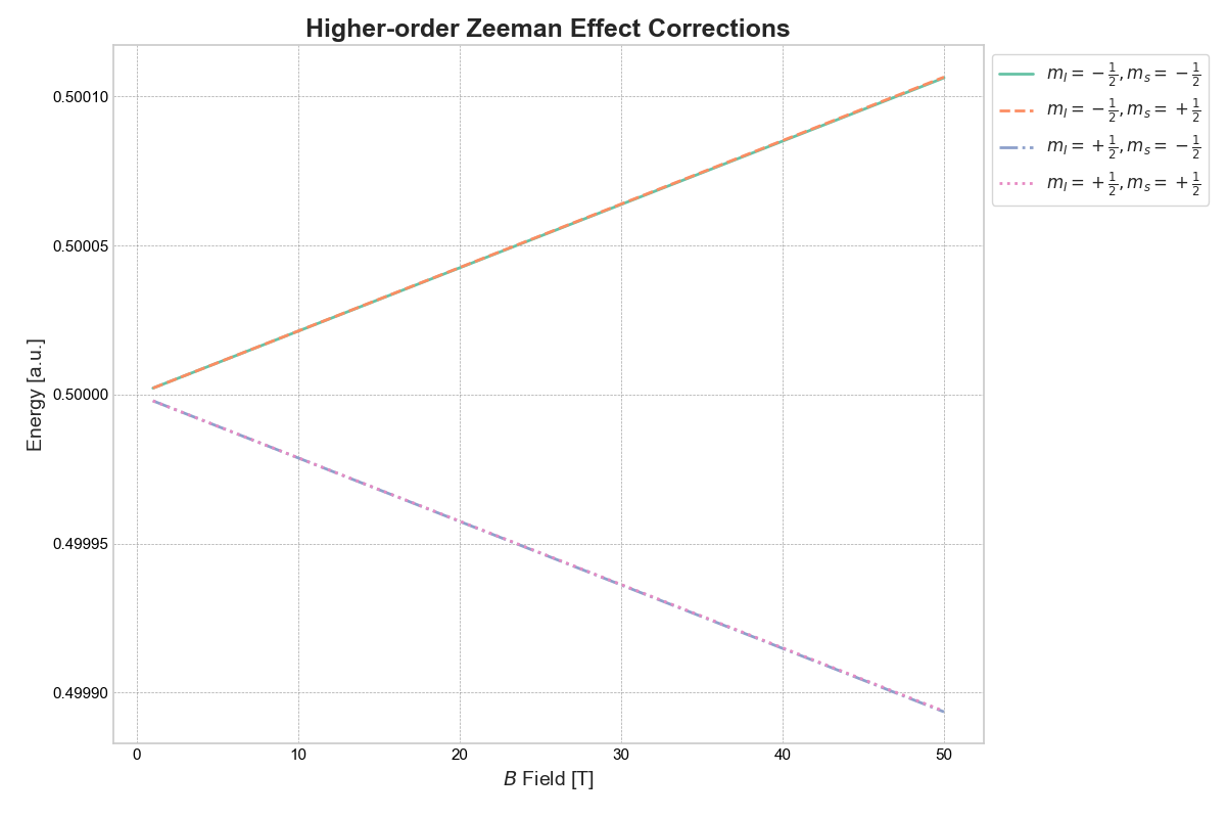
\includegraphics[width=0.85\linewidth]{Zeeman_Graph.png}
                \caption{The Zeeman splitting including all smaller corrections for $B=0T$ to $B=50T$. It can be seen that the higher order effects are sufficiently small, and the linear effects still dominate.}\label{fig:d}
            \end{center}
        \end{figure}
        \noindent The effect and its impact is shown in figure \ref{fig:d} and the result is also expressed numerically for any magnetic field strength and spin $\pm \frac{1}{2}$ as
        \begin{align}
            C_{\text{rel}}^{(2)} = \mp 1.677937685(16)\times 10^{-39} \cdot B^3\;.
        \end{align}
        \noindent Which has units of joules per tesla cubed $\left[J \cdot T^{-3}\right]$. Written in Hz at $1$T
        \begin{align}
            C_{\text{rel}}^{(2)} =2.532327297(39)\times 10^{-6} \text{  Hz.}
        \end{align}
        \noindent Comparing to the result at the Max Planck institute in Germany, a magnetic field strength of $B = 5.7T$
        \begin{align}
            C_{\text{rel}}^{(2)} = 3.107423136(16)\times10^{-37} J\;.
        \end{align}
        \noindent Or, written in Hz
        \begin{align}
            C_{\text{rel}}^{(2)} = 0.000468969(39) \text{  Hz.}
        \end{align}
        \noindent The accuracy of the high precision magnetometer at the Max Planck Institute has an accuracy which is approaching the sub ppb level, with most recent accuracy reported as $\pm 0.26$Hz \cite{Schneider_Sikora_Dickopf_Müller_Oreshkina_Rischka_Valuev_Ulmer_Walz_Harman_et_al._2022}. This calculated value is right on the cusp of an observable phenomenon, and will need to be accounted for if the accuracy of the experiment increases by only 2 orders of magnitude.